\documentclass[aspectratio=169,10pt]{beamer}

\makeatletter
\def\input@path{{jacquenetta/}}
\makeatother
\usetheme{JacquenettaMono}
\usepackage[utf8]{inputenc}
\usepackage{amsmath,amssymb,bm}
\usepackage{array,booktabs,tabularx}
\usepackage{adjustbox}
\usepackage{graphicx}
\usepackage{ragged2e}
\usepackage{tikz}
\usetikzlibrary{arrows.meta,calc,positioning}

\graphicspath{{figs/summer_recap_2026/}}

\title{Deep Teaching Guide: From Plasma Source Physics to Automated Shielding Design in Stellarators}
\author{Thaddaeus Kiker}
\institute{MIT Plasma Science and Fusion Center}
\date{August 26th, 2026}

\newcommand{\Bhat}{\widehat{\mathbf{B}}}
\newcommand{\uhat}{\widehat{\mathbf{u}}}
\newcommand{\rhat}{\widehat{\mathbf{r}}}
\newcommand{\dd}{\mathrm{d}}
\newcommand{\code}[1]{\texttt{\detokenize{#1}}}
\newcommand{\head}[1]{\par\vspace{0.08cm}{\fontsize{7.5}{9}\selectfont\color{jqgray}\MakeUppercase{#1}}\par\vspace{0.06cm}}
\newcommand{\src}[1]{\vfill\noindent\begin{adjustbox}{max width=\linewidth}{\fontsize{5.8}{7.1}\selectfont\color{jqgray}Evidence: \code{#1}}\end{adjustbox}\par\vspace{0.35cm}}
\newcommand{\srcpair}[2]{\vfill\noindent\begin{adjustbox}{max width=\linewidth}{\fontsize{5.8}{7.1}\selectfont\color{jqgray}Evidence: \code{#1}; \code{#2}}\end{adjustbox}\par\vspace{0.35cm}}
\newcommand{\claim}[1]{\par\vspace{0.10cm}\begin{minipage}{\linewidth}\color{jqdark}\vrule width 2.0pt\hspace{3mm}\begin{minipage}{\dimexpr\linewidth-2.0pt-3mm\relax}#1\end{minipage}\end{minipage}\par}
\newcommand{\twocol}[2]{\begin{columns}[t,onlytextwidth]\begin{column}{0.48\textwidth}#1\end{column}\begin{column}{0.48\textwidth}#2\end{column}\end{columns}}
\newcommand{\qtitle}[1]{{\fontsize{8}{10}\selectfont\color{jqgray}QUESTION}\par\vspace{0.06cm}{\fontsize{10.2}{12.8}\selectfont #1}\par\vspace{0.12cm}\rule{\linewidth}{0.55pt}\par\vspace{0.12cm}}
\newcommand{\answer}[1]{{\fontsize{8.7}{11.3}\selectfont #1}}
\newcommand{\notespace}{\par\vspace{0.08cm}{\color{jqlight}\rule{\linewidth}{0.4pt}}}

\begin{document}

{\setbeamertemplate{footline}{}
\begin{frame}[plain,noframenumbering]
  \vfill
  {\fontsize{19}{24}\selectfont Deep Teaching Guide\par}
  \vspace{0.25cm}
  {\fontsize{14}{19}\selectfont From Plasma Source Physics to Automated Shielding Design in Stellarators\par}
  \vspace{0.35cm}
  {\color{jqdark}\rule{\linewidth}{0.8pt}}
  \vspace{0.30cm}
  {\fontsize{9}{12}\selectfont Slide-by-slide physics, code, methods, claim boundaries, and oral-exam preparation\par}
  \vspace{0.12cm}
  {\fontsize{7.5}{10}\selectfont Prepared for the August 26th, 2026 presentation\par}
  \vfill
\end{frame}}

\begin{frame}{How to Use This Guide}
\small
Read the page with the same title as the talk slide immediately before rehearsing that slide. Pages marked (A), (B), and (C) expand one visible talk slide into the background you should know but should not try to say all at once.

\head{Three Levels of Certainty}
Implemented means the code path exists. Validated means a named numerical or statistical gate passed. Demonstrated means the method survived a transport calculation at the stated fidelity. Upstream means accepted into ordinary OpenMC development. These are different claims.

\head{Rehearsal Method}
First read for understanding. On the second pass, write a one-sentence answer to the page's main question. On the third pass, practice the compact answer aloud and keep the technical derivation for follow-up.

\claim{The objective is not memorization. It is to know which layer of the argument to reveal when somebody asks one level deeper.}
\src{spf_prototype/talk/summer_recap_2026-08-26_teaching_guide.md}
\end{frame}

% BEGIN INTRO CONTINUATION AND SECTION I
\begin{frame}{Claim Discipline Before Content}
\small
\head{What You Can Say}
You built an OpenMC-native stellarator source prototype, integrated one local-field SPF kernel with both Peterson's tokamak position sampler and a VMEC/DESC stellarator sampler, validated the angular physics and several transport limits, and assembled an end-to-end ParaStell--OpenMC shielding design loop.

\head{What You Must Qualify}
The source work is staged on a PR-\#3999-based tree rather than accepted upstream. The fifteen-geometry SPF result is free-streaming. The shielding result is a coarse finite-intervention study, not an optimum. The periodic wedge still needs an identically normalized full-torus validation. The exact attribution-to-worth comparison is unfinished.

\head{What You Must Not Say}
Do not claim the first VMEC stellarator source in Monte Carlo, a demonstrated factor-of-five design improvement, a converged Pareto front, or that FW-CADIS/SSR solved the runtime problem.
\srcpair{spf_prototype/talk/summer_recap_2026-08-26_teaching_guide.md}{spf_prototype/docs/notes/LIT_REVIEW_NOVELTY.md}
\end{frame}

\begin{frame}{Contents (A): The Argument of the Talk}
\scriptsize
\begin{enumerate}
  \setlength\itemsep{0.05cm}
  \item A credible optimization study needs a credible source: neutron births must follow the three-dimensional plasma volume and, for SPF, the local magnetic field.
  \item The local-field kernel changes both the neutron count and the angular distribution. The angular implementation can be validated much more strongly than a single end-result plot.
  \item Stellarator shielding is a spatial design field. Cheap geometric predictors were not reliable enough, so neutronics stays inside the design loop.
  \item The first coarse response matrix shows placement-dependent control, but engineering normalization, exact feasibility, independent reproduction, and convergence are still gates.
\end{enumerate}
\vspace{-0.08cm}
\claim{The argument is a chain: source fidelity $\rightarrow$ kernel validation $\rightarrow$ transport-informed shielding design.}
\end{frame}

\begin{frame}{Contents (B): The One-Sentence Thesis}
\vfill
\centering
\begin{minipage}{0.86\textwidth}
\fontsize{12}{17}\selectfont
A native equilibrium-aware plasma source makes local-field spin-polarized emission available inside OpenMC; once transport shows that source steering alone is not a reliable global shielding lever, the same source and geometry infrastructure become the forward model for response-aware nonuniform shielding design.
\end{minipage}
\vfill
\src{spf_prototype/talk/summer_recap_outline_2026-08-24.md}
\end{frame}

{\setbeamertemplate{footline}{}
\begin{frame}[plain,noframenumbering]
\vfill
{\fontsize{12}{14}\selectfont I\par}
\vspace{0.35cm}
{\fontsize{21}{27}\selectfont Native \texttt{StellaratorSource}\par in OpenMC\par}
\vspace{0.35cm}
{\fontsize{9}{12}\selectfont Study question: how do you sample the right place and the right local field without leaving the transport code?\par}
\vfill
\end{frame}}

\begin{frame}{Tokamaks vs. Stellarators: A Tale as Old as MCF (A)}
\small
\head{Geometric Distinction}
A tokamak is axisymmetric: one poloidal cross-section, rotated through toroidal angle $\phi$, generates the whole plasma. A stellarator deliberately breaks continuous axisymmetry; its surfaces vary with both poloidal angle $\theta$ and toroidal angle $\zeta$, while repeating after a finite number of field periods $N_{\mathrm{fp}}$.

\head{Source-Model Consequence}
Peterson's tokamak source can encode shape through a compact Miller-like parameterization. A general stellarator source cannot infer volume or field direction from one cross-section. It needs an equilibrium map over $(\rho,\theta,\zeta)$.

\head{Neutronics Consequence}
The neutron is uncharged after birth, but the magnetic field matters at birth because SPF emission is measured relative to the local $\Bhat$. Thus geometry and field enter the source even though they do not bend the neutron trajectory.
\srcpair{spf_prototype/native_spf/source.cpp}{spf_prototype/native_spf/stellarator_source.cpp}
\end{frame}

\begin{frame}{Tokamaks vs. Stellarators: A Tale as Old as MCF (B)}
\small
\centering
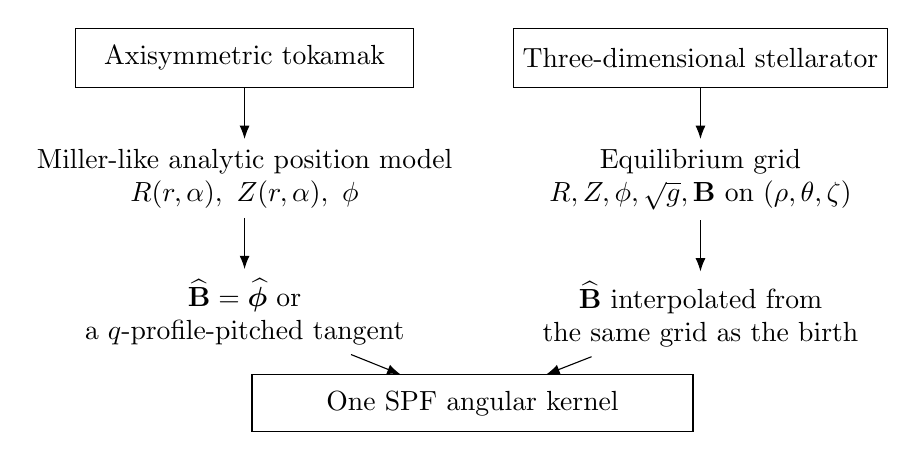
\begin{tikzpicture}[node distance=0.65cm and 1.0cm,>=Latex]
\node[draw,minimum width=4.3cm,minimum height=0.75cm] (tok) {Axisymmetric tokamak};
\node[draw,right=1.25cm of tok,minimum width=4.3cm,minimum height=0.75cm] (stel) {Three-dimensional stellarator};
\node[below=of tok,align=center] (tpos) {Miller-like analytic position model\\$R(r,\alpha),\ Z(r,\alpha),\ \phi$};
\node[below=of stel,align=center] (spos) {Equilibrium grid\\$R,Z,\phi,\sqrt{g},\mathbf B$ on $(\rho,\theta,\zeta)$};
\node[below=of tpos,align=center] (tb) {$\Bhat=\widehat{\boldsymbol\phi}$ or\\a $q$-profile-pitched tangent};
\node[below=of spos,align=center] (sb) {$\Bhat$ interpolated from\\the same grid as the birth};
\node[draw,below=0.78cm of $(tb)!0.5!(sb)$,minimum width=5.6cm,minimum height=0.72cm] (kernel) {One SPF angular kernel};
\draw[->] (tok)--(tpos); \draw[->] (stel)--(spos);
\draw[->] (tpos)--(tb); \draw[->] (spos)--(sb);
\draw[->] (tb)--(kernel); \draw[->] (sb)--(kernel);
\end{tikzpicture}
\vspace{0.18cm}
\claim{Two position models, two local-field models, one direction sampler. That is the clean architecture.}
\srcpair{spf_prototype/native_spf/README_apply.md}{spf_prototype/native_spf/README_stellarator.md}
\end{frame}

\begin{frame}{Building a General Stellarator Source in OpenMC (A)}
\small
\head{Lineage}
Peterson PR \#3999 supplies the native \texttt{TokamakSource} pattern: a Python \texttt{SourceBase} object serializes XML, C++ constructs a source object, and \texttt{sample(seed)} produces an OpenMC \texttt{SourceSite} inside the transport loop.

\head{Your Extension to the Tokamak Path}
The PR's Miller birth-position sampler remains intact. Your patch adds optional polarization plus a local field model: pure toroidal $\widehat{\boldsymbol\phi}$ or a Miller-surface poloidal tangent scaled by a supplied safety-factor profile $q(r/a)$.

\head{Your New Stellarator Path}
\texttt{StellaratorSource} is a sibling source class. It replaces the analytic position model with a gridded equilibrium sampler and obtains $\Bhat$ from the same map. It then calls the same SPF direction logic.
\claim{The strongest wording is “integrated with Peterson's PR-\#3999-based source architecture,” not “already upstream in OpenMC.”}
\srcpair{spf_prototype/native_spf/openmc_integration/README.md}{spf_prototype/native_spf/README_apply.md}
\end{frame}

\begin{frame}{Building a General Stellarator Source in OpenMC (B)}
\small
\head{Native Means More Than Python Syntax}
The source executes in C++ once per particle history. It uses \texttt{openmc::prn}, produces the same \texttt{SourceSite} fields as other OpenMC sources, is registered in \texttt{Source::create}, and uses OpenMC's XML and energy/time distributions.

\head{Files and Responsibilities}
\code{stellarator_source.cpp/.h} implement map I/O, CDF construction, interpolation, local-field evaluation, and sampling. \code{stellarator_source.py} validates user inputs and performs XML round trips. The integration patch touches CMake, source dispatch, Python exports, and Peterson's tokamak source.

\head{Backward Compatibility}
When \texttt{polarization=None}, no polarization XML is emitted and the C++ source takes the existing isotropic draw. That confines behavior change to opt-in input.
\src{spf_prototype/native_spf/openmc_integration/spf_core_integration.patch}
\end{frame}

\begin{frame}{Building a General Stellarator Source in OpenMC (C)}
\small
\head{Why Not Call Python from C++}
Source sampling is on the transport hot path and runs under OpenMP. A Python callback would impose interpreter overhead and the global interpreter lock. The production sampler therefore belongs in C++.

\head{Why Keep a Python Reference}
The Python \texttt{ConformalStellaratorSampler} is an executable specification. The C++ port preserves axis order, search convention, interpolation term order, periodic wrap, and random-number draw order. This permits deterministic parity checks rather than relying only on similar histograms.

\head{Current Maturity}
The canonical integrated snapshot exists and was used by the Ginsburg transport pipeline. Mirror-level tests pass. The remaining upstream-quality gate is a clean PR-\#3999-based build and native C++/Python seed parity and regression suite in the target checkout.
\srcpair{spf_prototype/python/stellarator_source.py}{spf_prototype/native_spf/test_stellarator_source_cpp.py}
\end{frame}

\begin{frame}{Integrating VMEC (I/II): Three-Dimensional Plasma Coordinates (A)}
\footnotesize
\head{Coordinates}
The equilibrium labels nested flux surfaces by $\rho$, position around a cross-section by $\theta$, and toroidal position by $\zeta$. The physical map is
\[
(\rho,\theta,\zeta)\mapsto \bigl(R(\rho,\theta,\zeta),\ Z(\rho,\theta,\zeta),\ \phi(\rho,\theta,\zeta)\bigr).
\]
The Cartesian position is $x=R\cos\phi$, $y=R\sin\phi$, $z=Z$.

\head{Volume Element}
Uniform sampling in coordinate space is not uniform sampling in physical volume. The volume element is
\[
\dd V=\left|\sqrt{g}(\rho,\theta,\zeta)\right|\dd\rho\,\dd\theta\,\dd\zeta.
\]
The source-cell weight is therefore $w_{ijk}=S(\rho_i)|\sqrt{g}_{ijk}|$, where $S$ is the radial emissivity profile.
\claim{Without $\sqrt{g}$, compressed coordinate regions are over-sampled and the wall-load pattern is biased before transport begins.}
\src{spf_prototype/python/stellarator_source.py}
\end{frame}

\begin{frame}{Integrating VMEC (I/II): Three-Dimensional Plasma Coordinates (B)}
\footnotesize
\head{Flux-Map Contract}
The portable \code{spf_fluxmap_v1} input contains one text metadata file and one little-endian \texttt{float64} payload. The payload order is fixed:
\[
\rho,\theta,\zeta,\sqrt{g},R,Z,\phi,B_R,B_\phi,B_Z.
\]
Every three-dimensional array uses C order with indices $[i_\rho,j_\theta,k_\zeta]$.

\head{Why a Small Binary Format}
The C++ reader uses \texttt{std::ifstream} and adds no HDF5 dependency to the source implementation. The format is producer-agnostic: DESC, VMEC, or a synthetic analytic torus can write the same contract.

\head{Important Convention}
$\theta$ and $\zeta$ cover $[0,2\pi)$ and wrap periodically. $\rho$ excludes the magnetic axis, where $\sqrt{g}\rightarrow0$, and is treated as nonperiodic.
\src{spf_prototype/native_spf/README_stellarator.md}
\end{frame}

\begin{frame}{Integrating VMEC (I/II): Three-Dimensional Plasma Coordinates (C)}
\footnotesize
\head{Rejection-Free Cascade}
The normalized joint distribution is factored as
\[
p(\rho,\theta,\zeta)=p(\rho)\,p(\zeta\mid\rho)\,p(\theta\mid\rho,\zeta).
\]
Three CDFs are precomputed: a marginal radial CDF, a conditional toroidal CDF for each radial shell, and a conditional poloidal CDF for each $(\rho,\zeta)$ pair.

\head{Sampling Order}
Cell selection consumes three draws in the exact order $\rho\rightarrow\zeta\rightarrow\theta$. It uses \code{upper_bound}, equivalent to NumPy \code{searchsorted(side="right")-1}, then clamps to valid cells.

\head{Why This Matters}
Every accepted birth has spatial weight one. There is no rejection-efficiency penalty in strongly nonuniform three-dimensional geometry, and no variable source weight from spatial sampling.
\srcpair{spf_prototype/native_spf/stellarator_source.cpp}{spf_prototype/native_spf/test_stellarator_source_cpp.py}
\end{frame}

\begin{frame}{Integrating VMEC (I/II): Three-Dimensional Plasma Coordinates (D)}
\small
\head{Grid-to-Continuous Birth}
After a cell is selected, three new uniforms jitter $\rho$, $\theta$, and $\zeta$ inside the cell. The source then trilinearly interpolates the geometry fields. $\rho$ uses a clamped bracket; $\theta$ and $\zeta$ wrap modulo $2\pi$.

\head{Subtle Edge Behavior}
Jitter may place $\rho$ half a grid cell beyond the first or last stored node. The bracket is clamped, so this is bounded extrapolation rather than an out-of-bounds access. The discretization bias vanishes with radial grid refinement. It is documented because an upstream reviewer will ask.

\head{Interpolation Order}
The C++ arithmetic order matches the Python reference: interpolate in $\theta$, then $\zeta$, then $\rho$. Matching algebraic order helps deterministic parity by limiting floating-point re-association.
\src{spf_prototype/native_spf/stellarator_source.cpp}
\end{frame}

\begin{frame}{Integrating VMEC (II/II): Neutron Birth and Local $\Bhat$ (A)}
\footnotesize
\head{Same-Map Consistency}
At the sampled $(\rho,\theta,\zeta)$, the source interpolates $B_R$, $B_\phi$, and $B_Z$ from the same equilibrium grid used for $R$, $Z$, and $\phi$. Cylindrical components are rotated to Cartesian:
\[
B_x=B_R\cos\phi-B_\phi\sin\phi,\qquad
B_y=B_R\sin\phi+B_\phi\cos\phi,
\]
then $\mathbf B$ is normalized.

\head{Why Same-Map Matters}
Sampling position from one equilibrium and field direction from an unrelated approximation would create a physically inconsistent polarization axis. Here the source location, metric Jacobian, and $\Bhat$ share one grid and one interpolation point.

\head{Axisymmetric Override}
\code{field_model='toroidal'} replaces the grid field with $\widehat{\boldsymbol\phi}=(-\sin\phi,\cos\phi,0)$, providing a clean limit for comparison with the tokamak and analytic oracles.
\src{spf_prototype/native_spf/stellarator_source.cpp}
\end{frame}

\begin{frame}{Integrating VMEC (II/II): Neutron Birth and Local $\Bhat$ (B)}
\small
\head{Tokamak Local Field}
For Peterson's source, the pitched option forms a unit poloidal tangent from Miller-surface derivatives and combines it with the toroidal direction:
\[
\mathbf B\propto\widehat{\boldsymbol\phi}+s\lambda\widehat{\mathbf p},
\qquad \lambda=\frac{r}{q(r/a)R}.
\]
The sign $s=\pm1$ controls handedness. As $q\rightarrow\infty$, $\lambda\rightarrow0$ and the field becomes toroidal.

\head{Stellarator Local Field}
The stellarator path does not approximate pitch from $q$. It reads all three field components from the equilibrium map. This is the essential local-field generalization.

\head{Shared Contract}
Both position samplers hand one normalized vector $\Bhat$ to the direction kernel. The kernel never needs to know whether the point came from Miller coordinates or VMEC coordinates.
\src{spf_prototype/native_spf/source.cpp}
\end{frame}

\begin{frame}{StellaratorSource Validation (I/II) (A)}
\small
\head{Producer Gates}
Before a flux map is written, the pipeline checks equilibrium convergence, single-signed $\sqrt{g}$ on nested surfaces, tensor-grid ordering, LCFS reconstruction, and volume by two routes: direct $\sqrt{g}$ quadrature and an independent divergence-theorem surface integral.

\head{Why Two Volume Tests}
Agreement with the equilibrium code's stored volume can miss a shared convention error. The divergence-theorem calculation uses different geometry and numerical structure, so agreement is a stronger guard against axis ordering, sign, or coordinate mistakes.

\head{Failure Policy}
These are generation-time gates. A map that fails is not allowed to reach the source sampler. That is more defensible than warning and proceeding with an unphysical coordinate system.
\srcpair{spf_prototype/python/quasr_fluxmap.py}{spf_prototype/native_spf/README_stellarator.md}
\end{frame}

\begin{frame}{StellaratorSource Validation (I/II) (B)}
\footnotesize
\head{Synthetic Circular-Torus Oracle}
For
\[
R=R_0+a\rho\cos\theta,\qquad Z=a\rho\sin\theta,\qquad \phi=\zeta,
\]
the physical Jacobian is known exactly:
\[
\sqrt{g}=R\,a^2\rho.
\]
Choosing $B_\phi\propto1/R$ and $B_R=B_Z=0$ also gives a known $\Bhat=\widehat{\boldsymbol\phi}$.

\head{What This Oracle Isolates}
It tests the map format, CDF axes, cell selection, interpolation, coordinate conversion, field rotation, normalization, unit source weight, and periodic wrap without depending on a difficult external equilibrium.

\head{Observed Agreement}
CDFs agree with the NumPy reference near $10^{-12}$; sampled positions and $\Bhat$ agree near $10^{-10}$ in the mirror tests.
\srcpair{spf_prototype/python/stellarator_source.py}{spf_prototype/native_spf/test_stellarator_source_cpp.py}
\end{frame}

\begin{frame}{StellaratorSource Validation (II/II) (A)}
\small
\head{Three Validation Layers}
Layer one validates source algebra and RNG parity without transport. Layer two uses near-void OpenMC transport to compare neutron wall loading with analytic quadrature. Layer three turns material scattering on and checks physically new observables such as down-scattered spectra, heating, and TBR.

\head{Why Free Streaming Is Powerful}
In the near-void limit, OpenMC should reproduce a direct line-of-sight integral. Any coherent discrepancy points to source direction, geometry, tally, or normalization—not complicated material physics.

\head{Why Scattering Comes Later}
Once the zero-scattering limit is pinned, differences after materials are enabled become interpretable as transport physics rather than implementation uncertainty.
\src{spf_prototype/docs/notes/results/JOINT_VALIDATION.md}
\end{frame}

\begin{frame}{StellaratorSource Validation (II/II) (B)}
\small
\head{Quadrature Check}
The independent analytic engine evaluates the free-streaming wall-load integral with Gauss--Legendre quadrature. For the square-torus benchmark it agrees with Schwartz's \texttt{anarrima} expressions to $5.2\times10^{-8}$ across the plasma-wall pattern and to machine precision for single rings.

\head{Transport Check}
Four million OpenMC histories per mode reproduce the analytic mode-to-isotropic patterns. Standardized residuals have means near zero; their widths are no larger than order unity, consistent with Monte Carlo uncertainty rather than a coherent bias.

\head{Real-Geometry Check}
On QUASR 59509's conformal wall, analytic point-patch and ray-traced OpenMC results agree by roughly $0.5$--$2.3\%$ regionally, with the largest residual on the close, curved inboard wall.
\srcpair{spf_prototype/docs/notes/results/RESULTS_tier2b.md}{spf_prototype/paper/data/conformal_xcheck.csv}
\end{frame}

\begin{frame}{StellaratorSource Validation (II/II) (C)}
\small
\head{What Is Validated Today}
The spatial reference algorithm, map round trip, CDF cascade, interpolation, field direction, unit weight, angular statistics, analytic wall-load limit, and several scattering observables all have named tests or recorded results.

\head{What Is Still a Build-Time Gate}
The staging documentation still calls for a native, identical-seed C++ \texttt{openmc::prn} parity dump in the exact integrated checkout, followed by the PR-\#3999 regression suite. Mirror parity is strong evidence, but upstream reviewers will want the built artifact itself exercised.

\head{How to Answer “Is It Paper-Ready?”}
The scientific core is substantial enough for a source-method paper. Publication strength depends on closing integration regression gates, documenting grid convergence, expanding source profiles/energy treatment, and presenting a clean upstream-quality API and comparison set.
\srcpair{spf_prototype/native_spf/README_stellarator.md}{spf_prototype/docs/writeups/stellarator_source_eval.tex}
\end{frame}

% BEGIN SECTION II
{\setbeamertemplate{footline}{}
\begin{frame}[plain,noframenumbering]
\vfill
{\fontsize{12}{14}\selectfont II\par}
\vspace{0.35cm}
{\fontsize{21}{27}\selectfont Spin-Polarized Plasma\par Neutronics\par}
\vspace{0.35cm}
{\fontsize{9}{12}\selectfont Study question: how do spin-state populations become a correctly normalized local-field neutron source?\par}
\vfill
\end{frame}}

\begin{frame}{Overview of Spin-Polarized Fusion (A)}
\footnotesize
\head{Reaction}
For deuterium--tritium fusion,
\[
{}^2\mathrm D+{}^3\mathrm T\rightarrow{}^4\mathrm{He}\,(3.5\ \mathrm{MeV})+n\,(14.1\ \mathrm{MeV}).
\]
Preparing nuclear spin populations changes the allowed entrance-channel mixture. That affects the total reaction rate and the neutron angular distribution relative to the quantization axis, taken here as the local magnetic field.

\head{Three Collision-Mode Fractions}
The spin populations map to $a$, $b$, and $c$:
\[
a=d_+t_+ + d_-t_-,\qquad b=d_0,\qquad c=d_+t_-+d_-t_+.
\]
For unpolarized fuel, $a=b=c=1/3$.

\claim{The source input may be physical spin fractions or the derived $(a,b,c)$ mixture. The transport kernel uses the latter.}
\srcpair{spf_prototype/native_spf/source.py}{spf_prototype/python/abc_modes.py}
\end{frame}

\begin{frame}{Overview of Spin-Polarized Fusion (B)}
\footnotesize
\head{Two Angular Shapes}
Although there are three collision fractions, there are only two distinct neutron angular shapes:
\[
f_\perp(x)\propto 1-x^2,\qquad
f_\parallel(x)\propto \frac14+\frac34x^2,
\qquad x=\uhat\cdot\Bhat.
\]
The $a$ contribution uses the perpendicular-peaked shape. Both $b$ and $c$ use the same parallel-peaked shape.

\head{Expected Second Moments}
The most useful scalar oracle is
\[
\left\langle x^2\right\rangle=
\begin{cases}
1/5,&\text{pure }a,\\
1/3,&\text{unpolarized},\\
7/15,&\text{pure }b\text{ or }c.
\end{cases}
\]
These values distinguish oblate, isotropic, and prolate emission about $\Bhat$ without depending on a particular global coordinate axis.
\src{spf_prototype/docs/notes/results/RESULTS_tier1.md}
\end{frame}

\begin{frame}{Overview of Spin-Polarized Fusion (C)}
\small
\head{Nematic Rather Than Vector Anisotropy}
The kernels depend on $x^2=(\uhat\cdot\Bhat)^2$, so reversing $\Bhat$ does not change the distribution. The angular preference is an axis, not an arrow. This is why a second-rank $P_2$ description is natural.

\head{Legendre Form}
After normalization, the directional density can be written
\[
p(\uhat\mid\Bhat)=\frac{1}{4\pi}\left[1+a_2P_2(\uhat\cdot\Bhat)\right],
\qquad P_2(x)=\frac{3x^2-1}{2},
\]
with $a_2=-1$ for pure $a$, $a_2=0$ for unpolarized fuel, and $a_2=+1$ for pure $b/c$ directionality.

\head{Interpretation}
$a_2<0$ favors directions broadside to the field; $a_2>0$ favors directions along either sign of the field axis.
\src{spf_prototype/docs/teaching/spf_order_parameter_teaching_deck.tex}
\end{frame}

\begin{frame}{Spin-Polarized Fusion Changes Rate and Emission Angle (A)}
\small
\head{Differential Cross Section}
The implemented Schwartz form is
\[
\frac{\dd\sigma}{\dd\Omega}=\frac{\sigma_0}{2\pi}
\left[
\frac34a\sin^2\vartheta+
\left(\frac23b+\frac13c\right)
\left(\frac14+\frac34\cos^2\vartheta\right)
\right],
\]
where $\vartheta$ is measured from the local $\Bhat$.

\head{Sampler Coefficients}
Define $w_\perp=3a/4$ and $w_\parallel=2b/3+c/3$. Their solid-angle integrals are not equal, so the mixture-selection probability is not simply $w_\perp/(w_\perp+w_\parallel)$.

\head{Key Separation}
The normalized angular PDF controls where neutrons go. The integral of the differential cross section controls how many neutrons are produced at fixed fuel density.
\src{spf_prototype/native_spf/source.cpp}
\end{frame}

\begin{frame}{Spin-Polarized Fusion Changes Rate and Emission Angle (B)}
\small
\head{Derive the Rate Factor}
Using
\[
\int\sin^2\vartheta\,\dd\Omega=\frac{8\pi}{3},\qquad
\int\left(\frac14+\frac34\cos^2\vartheta\right)\dd\Omega=2\pi,
\]
the total reaction-rate factor is
\[
\eta=a+\frac23b+\frac13c.
\]
The probability of selecting the perpendicular angular family is
\[
P_\perp=\frac{2\pi a}{2\pi a+2\pi w_\parallel}=\frac{a}{\eta}.
\]

\head{Corner Rates Relative to Unpolarized Fuel}
Unpolarized has $\eta=2/3$. Pure $a$ has $\eta=1$ and therefore $1.5$ times the rate. Pure $b$ retains the unpolarized rate. Pure $c$ has $\eta=1/3$ and therefore half the rate.
\srcpair{spf_prototype/tests/test_abc_modes.py}{spf_prototype/docs/notes/results/RESULTS_tier7.md}
\end{frame}

\begin{frame}{Spin-Polarized Fusion Changes Rate and Emission Angle (C)}
\small
\head{Why Constant-Rate Comparisons Exist}
To validate directionality, each sampled angular distribution is normalized to one neutron per source history. Mode-to-isotropic wall-load ratios then isolate steering and are independent of $\eta$.

\head{Why Rate Must Return Later}
At fixed fuel density, the physical source strength must be multiplied by $\eta/(2/3)$. Otherwise pure $a$'s $50\%$ rate gain and pure $c$'s rate penalty disappear from engineering comparisons.

\head{A Useful Oral Answer}
“I separated the conditional direction PDF from the scalar fusion-rate factor. The Monte Carlo sampler validates the directional kernel at constant neutron count; systems or absolute-load calculations restore $\eta$.”

\claim{Do not call a constant-rate wall-load ratio an absolute reactor-load prediction.}
\src{spf_prototype/paper/data/rate_steering.csv}
\end{frame}

\begin{frame}{Prior Spin-Polarized Fusion Neutronics (A)}
\small
\head{Schwartz}
Schwartz supplies the axisymmetric analytic wall-loading theory and the $(a,b,c)$ angular parameterization. The theory is differentiable and exact for its free-streaming, convex, axisymmetric assumptions. It does not include material scattering.

\head{Bae et al.}
Bae and collaborators performed OpenMC neutronics for spin-polarized spherical tokamak concepts. Their work already establishes that polarized source direction can affect center-stack loading and TBR in a tokamak.

\head{Your Defensible Distinction}
Your source is native and generated on the fly, accepts a spatially varying local field, and supports both Peterson's parametric tokamak birth model and a real-equilibrium stellarator birth model. The novelty is not “first polarized source in OpenMC.”
\src{spf_prototype/docs/notes/LIT_REVIEW_NOVELTY.md}
\end{frame}

\begin{frame}{Prior Spin-Polarized Fusion Neutronics (B)}
\small
\head{What the Literature Screenshots Are Doing}
They establish two independent anchors before your implementation details: an analytic directional oracle and a prior transport demonstration. This prevents the talk from presenting a known physical effect as if it were newly discovered.

\head{Validation Use}
Schwartz's rounded headline values are approximately $+43\%$ inboard and $-22\%$ outboard for the perpendicular-emitting mode at constant fusion rate. The exact \texttt{anarrima} example gives $+40.6\%$ and $-21.2\%$ for the stated geometry.

\head{Interpretation Use}
Bae's TBR trend supplies an external sign check: parallel-emitting cases modestly increase TBR and perpendicular-emitting cases modestly reduce it in their model. Your FLiBe box-torus reproduces the trend, not the exact magnitude.
\srcpair{spf_prototype/docs/notes/results/RESULTS_tier2a.md}{spf_prototype/docs/notes/results/RESULTS_tier6.md}
\end{frame}

\begin{frame}{Proposed StellaratorSource Interface for OpenMC (A)}
\small
\head{Python-Facing Inputs}
The prototype accepts a flux-map stem, optional polarization, field model, energy distribution, time distribution, radial emission profile, source strength, and ordinary OpenMC source constraints.

\head{Polarization Input}
Users may supply $(a,b,c)$ directly or a dictionary of deuteron and triton spin fractions. Inputs are checked for nonnegativity and positive sum, then renormalized with a warning if necessary.

\head{Defaults}
No polarization means an isotropic angle. The stellarator field model defaults to the flux map. Energy defaults to a $14.06\ \mathrm{MeV}$ discrete source; time defaults to zero; emissivity defaults to $S(\rho)=1-\rho^2$.
\src{spf_prototype/native_spf/stellarator_source.py}
\end{frame}

\begin{frame}{Proposed StellaratorSource Interface for OpenMC (B)}
\small
\head{XML Contract}
The Python object writes \texttt{fluxmap}, optional radial emission arrays, energy/time distributions, and—only if present—\texttt{polarization} and \code{field_model}. The C++ constructor validates the same physical invariants again.

\head{Why Validate Twice}
Python provides early, user-friendly errors. C++ protects correctness when XML is authored elsewhere or a caller bypasses the Python layer.

\head{Potential Upstream Review Point}
The bespoke binary is simple and dependency-free, but maintainers may prefer an established OpenMC HDF5 or mesh-field representation. Treat the file format as an explicit design choice open to review, not an immutable part of the physics.

\claim{The API should expose physical choices while keeping source-internal implementation details—CDF tables and frames—private.}
\srcpair{spf_prototype/native_spf/stellarator_source.py}{spf_prototype/native_spf/stellarator_source.cpp}
\end{frame}

\begin{frame}{One Kernel Supports Tokamak and Stellarator Sources (A)}
\footnotesize
\head{Kernel Inputs}
The direction sampler needs only $(a,b,c)$, a normalized local $\Bhat$, and an OpenMC RNG seed. It does not own geometry, plasma coordinates, or equilibrium evaluation.

\head{Kernel Output}
It returns one unit vector $\uhat$ distributed according to the normalized polarized angular density. Energy and time remain separate OpenMC distributions.

\head{Architectural Benefit}
The difficult angular physics and its validation are written once. Future source classes—a tabulated kinetic source, a time-dependent source, or a different confinement geometry—can reuse the same kernel if they supply $\Bhat$ at birth.

\head{Current Code Caveat}
The staging snapshot duplicates helper code between source translations. A polished upstream patch should factor the shared sampler into one tested internal component.
\srcpair{spf_prototype/native_spf/source.cpp}{spf_prototype/native_spf/stellarator_source.cpp}
\end{frame}

\begin{frame}{One Kernel Supports Tokamak and Stellarator Sources (B)}
\small
\centering
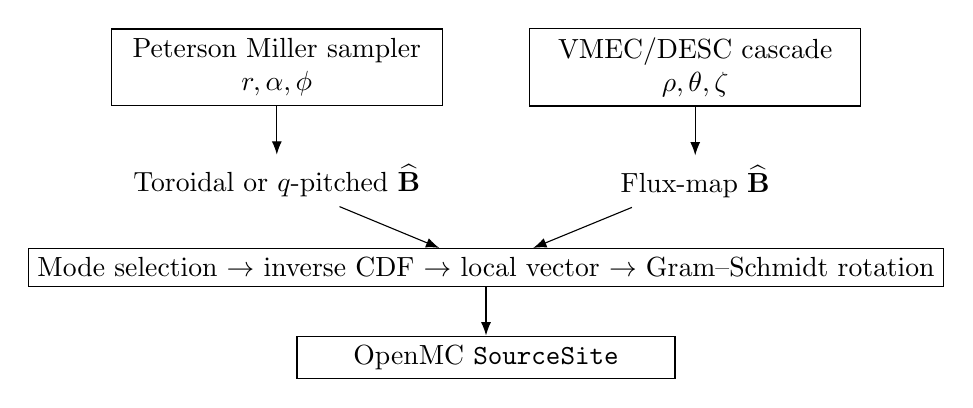
\begin{tikzpicture}[>=Latex,node distance=0.62cm and 1.1cm]
\node[draw,align=center,minimum width=4.2cm] (tp) {Peterson Miller sampler\\$r,\alpha,\phi$};
\node[draw,right=of tp,align=center,minimum width=4.2cm] (sp) {VMEC/DESC cascade\\$\rho,\theta,\zeta$};
\node[below=of tp,align=center] (tb) {Toroidal or $q$-pitched $\Bhat$};
\node[below=of sp,align=center] (sb) {Flux-map $\Bhat$};
\node[draw,below=0.85cm of $(tb)!0.5!(sb)$,align=center,minimum width=6.6cm] (k) {Mode selection $\rightarrow$ inverse CDF $\rightarrow$ local vector $\rightarrow$ Gram--Schmidt rotation};
\node[draw,below=of k,align=center,minimum width=4.8cm] (site) {OpenMC \texttt{SourceSite}};
\draw[->] (tp)--(tb); \draw[->] (sp)--(sb);
\draw[->] (tb)--(k); \draw[->] (sb)--(k); \draw[->] (k)--(site);
\end{tikzpicture}
\vspace{0.18cm}
\claim{The local-field interface is the reusable abstraction.}
\src{spf_prototype/native_spf/openmc_integration/README.md}
\end{frame}

\begin{frame}{SPF Kernel Validation (I/III) (A)}
\scriptsize
\head{Exact Shape Sampling}
Let $x=\cos\vartheta$. For the perpendicular family, inversion of the normalized CDF requires solving
\[
x^3-3x+(4u-2)=0.
\]
The in-range trigonometric root is
\[
x=2\cos\left[\frac13\arccos(1-2u)-\frac{2\pi}{3}\right].
\]
For the parallel family, inversion requires
\[
x^3+x+(2-4u)=0,
\]
which has one real Cardano root because its discriminant is positive.

\head{Why Inverse CDF}
It uses a fixed number of random draws and avoids rejection-loop divergence between implementations, which is valuable for exact seed parity and predictable source cost.
\src{spf_prototype/python/spf_mirror.py}
\end{frame}

\begin{frame}{SPF Kernel Validation (I/III) (B)}
\small
\head{Statistical Gates}
One million samples per configuration were compared with the analytic $x$ distribution. The observed $\chi^2$ per degree of freedom ranged from roughly $0.70$ to $1.37$ across unpolarized, pure modes, and a mixed mode; all recorded $p$-values exceeded $0.06$.

\head{Independent Sampler Check}
The inverse-CDF results were compared with a rejection sampler using a two-sample Kolmogorov--Smirnov test. The perpendicular and parallel shape comparisons had $p=0.102$ and $p=0.687$, respectively.

\head{Azimuth and Moments}
The azimuth around $\Bhat$ is uniform, and observed $\langle x^2\rangle$ matches $1/5$, $1/3$, and $7/15$ within a few $10^{-4}$ to $10^{-3}$.
\src{spf_prototype/docs/notes/results/RESULTS_tier1.md}
\end{frame}

\begin{frame}{SPF Kernel Validation (II/III) (A)}
\small
\head{Local-to-Global Rotation}
The sampler first creates
\[
\mathbf u_{\mathrm{local}}=
\left(\sqrt{1-x^2}\cos\varphi,\sqrt{1-x^2}\sin\varphi,x\right)
\]
in a frame whose third axis is $\Bhat$. To build the other axes robustly, choose the world basis vector least aligned with $\Bhat$, subtract its projection, normalize to obtain $\mathbf e_x$, then set $\mathbf e_y=\Bhat\times\mathbf e_x$.

\head{Why the Least-Aligned Axis}
Using a fixed reference such as $\widehat{\mathbf z}$ fails when $\Bhat\parallel\widehat{\mathbf z}$. The least-aligned choice bounds the Gram--Schmidt denominator away from zero.

\head{Invariant}
After rotation, $\uhat\cdot\Bhat=x$ and $\lVert\uhat\rVert=1$ to floating-point precision.
\src{spf_prototype/native_spf/source.cpp}
\end{frame}

\begin{frame}{SPF Kernel Validation (II/III) (B)}
\small
\head{Deterministic Parity}
The standalone C++ sampler and the Python mirror use an identical seed stream and draw order: family selector, inverse-CDF uniform, then azimuth. For 5,000 mixed-mode samples about an off-axis field, the recorded maximum component difference is $6.1\times10^{-16}$.

\head{Rotation Tests}
An isotropic distribution remains isotropic after rotation to an off-axis field. Pure-mode steering retains the analytic second moment. Explicit $\Bhat=\pm\widehat{\mathbf z}$ cases remain finite and correct.

\head{What This Proves}
The parity test detects algebraic transcription, RNG, and frame-rotation differences. The distribution tests detect a shared but mathematically wrong implementation. Together they are much stronger than either alone.
\srcpair{spf_prototype/tests/test_sampler_stats.py}{spf_prototype/docs/notes/results/RESULTS_tier1.md}
\end{frame}

\begin{frame}{SPF Kernel Validation (III/III) (A)}
\small
\head{Analytic Wall-Load Oracle}
For a wall point $\mathbf r_w$ and source point $\mathbf r_s$, the free-streaming contribution has inverse-square dilution, a projected-area factor, and the angular kernel evaluated at
\[
\widehat{\Delta}=\frac{\mathbf r_w-\mathbf r_s}{\lVert\mathbf r_w-\mathbf r_s\rVert},
\qquad x=\Bhat(\mathbf r_s)\cdot\widehat{\Delta}.
\]
Gauss--Legendre quadrature integrates this over the plasma source. The benchmark geometry also has Schwartz's closed-form/\texttt{anarrima} evaluation.

\head{Three-Engine Logic}
Quadrature versus \texttt{anarrima} validates the analytic reference. OpenMC versus quadrature validates the sampled source and transport wiring. Agreement among all three avoids circular validation.
\srcpair{spf_prototype/python/analytic_nwl.py}{spf_prototype/tests/test_analytic_nwl.py}
\end{frame}

\begin{frame}{SPF Kernel Validation (III/III) (B)}
\small
\head{Schwartz Recovery}
In the constant-rate square-torus case, OpenMC gives approximately $+39.2\%$ inboard and $-21.0\%$ outboard for pure perpendicular emission, compared with analytic $+40.6\%$ and $-21.2\%$. Parallel $b/c$ emission gives the opposite pattern.

\head{Bae Trend Recovery}
In the FLiBe blanket model, TBR per neutron is $1.149$ unpolarized, $1.144$ perpendicular, and $1.155$ parallel. This reproduces Bae et al.'s sign—parallel slightly up, perpendicular slightly down—while using a different breeder and scoping geometry.

\head{How to Phrase It}
“I recover Schwartz's axisymmetric wall-loading response and independently reproduce the direction of Bae's TBR change; I do not claim a pointwise reproduction of Bae's reactor.”
\srcpair{spf_prototype/docs/notes/results/RESULTS_tier2b.md}{spf_prototype/docs/notes/results/RESULTS_tier6.md}
\end{frame}

\begin{frame}{SPF Effects (I/II): $R$ and NWL Coupling (A)}
\small
\head{Constant-Rate Directionality}
At fixed neutron count, pure $a$ steers neutrons broadside to $\Bhat$ and can raise inboard wall load in a toroidal field. Pure $b/c$ favors the field axis and tends to reduce inboard load while raising outboard load.

\head{Fixed-Fuel-Density Reality}
The total load is the directional response multiplied by the rate factor. In the Tier-7 scoping model, pure $a$ produces $1.5$ times the fusion rate and compounds the inboard steering, yielding about $1.70$ times the center-stack load. Pure $b$ retains the original rate and lowers center-stack load to about $0.85$.

\head{Engineering Interpretation}
Pure $b$ is the rate-preserving steering state in this parameterization. Pure $c$ steers similarly but halves the absolute rate relative to unpolarized fuel.
\src{spf_prototype/paper/data/rate_steering.csv}
\end{frame}

\begin{frame}{SPF Effects (I/II): $R$ and NWL Coupling (B)}
\small
\head{Scattering Dilution}
In the thin-wall limit, perpendicular emission changes inboard/outboard loading by about $+40\%/-20\%$. With the W/steel/Be/FLiBe blanket active, the changes fall to approximately $+13.2\%/-9.2\%$.

\head{Physical Mechanism}
The anisotropy is imposed only at birth. Uncollided neutrons retain it; collisions redirect particles and generate a more diffuse return population. The transported wall load is therefore a mixture of a steered first-flight component and a partially isotropized collided component.

\head{Why Transport Matters}
The analytic free-streaming prediction is not wrong; it answers a different limit. OpenMC quantifies how much of that ideal steering survives realistic material interactions.
\claim{In this model, free-streaming overstates the retained directional lever by roughly a factor of three.}
\src{spf_prototype/docs/notes/results/RESULTS_tier5.md}
\end{frame}

\begin{frame}{SPF Effects (II/II): Poor Peaking Reduction by Geometry (A)}
\small
\head{Fifteen-Geometry Experiment}
Fifteen distinct QUASR equilibria were given the same conformal-wall rule and sampled with the native stellarator source. Each case produced free-streaming wall maps for unpolarized, perpendicular, and parallel emission. These are fifteen geometries, not fifteen walls on one reactor.

\head{Response Definition}
For each geometry,
\[
\mathrm{PF}=\frac{\max Q}{\langle Q\rangle_A},\qquad
Y=\frac{\mathrm{PF}_{\mathrm{unpol}}-\min_{a_2}\mathrm{PF}(a_2)}{\mathrm{PF}_{\mathrm{unpol}}}.
\]
The optimized $a_2$ is a continuous interpolation within the $P_2$ family, not a separately transported arbitrary angular distribution.

\head{Result Scale}
$Y$ spans roughly $0$--$16\%$ with a median near $4\%$.
\srcpair{spf_prototype/paper/data/predictor_n15.csv}{spf_prototype/paper/data/PROVENANCE.md}
\end{frame}

\begin{frame}{SPF Effects (II/II): Poor Peaking Reduction by Geometry (B)}
\small
\head{Why the Global Benefit Is Modest}
Many wall maps are dominated by a narrow grazing/near-field spike occupying only a small fraction of area. A smooth quadrupolar angular lever can shift broad inboard/outboard loading but cannot easily erase a geometry-created singular-looking maximum.

\head{Cheap Predictors}
The best of the tested simple descriptors was the inverse-square geometry headroom $\mathrm{PF}_{\mathrm{geo}}$, with Spearman $\rho\approx0.525$. Nematic wall-normal coherence had $\rho\approx0.396$, and shaping amplitude was weaker. At $n=15$, none is a reliable quantitative predictor.

\head{Takeaway}
SPF remains a physically meaningful local actuator and may protect a specific component, but it is not a dependable global wall-load flattener across stellarator geometry.
\srcpair{spf_prototype/talk/QA_RESEARCH.md}{spf_prototype/python/predictor_test.py}
\end{frame}

\begin{frame}{SPF Effects (II/II): Poor Peaking Reduction by Geometry (C)}
\small
\head{Statistical Summary to Know}
The benefit distribution is best described with median, interquartile range, and maximum rather than only a single mean. The main deck emphasizes the median near $4\%$ and the upper end near $16\%$; use the frozen CSV if somebody asks for a specific device.

\head{Sampling Caveat}
The set spans aspect ratio and shaping but is dominated by QA cases because strongly shaped QH equilibria often failed the fixed-boundary VMEC/conformal-wall pipeline. It is a useful diverse set, not an unbiased census of all stellarators.

\head{Fidelity Caveat}
These are first-flight/free-streaming maps. Scattering generally reduces directional contrast, so this result is closer to an upper-bound study of source steering than a reactor-final result.
\srcpair{spf_prototype/talk/QA_RESEARCH.md}{spf_prototype/paper/data/PROVENANCE.md}
\end{frame}

% BEGIN SECTION III
{\setbeamertemplate{footline}{}
\begin{frame}[plain,noframenumbering]
\vfill
{\fontsize{12}{14}\selectfont III\par}
\vspace{0.35cm}
{\fontsize{21}{27}\selectfont Automatic Reactor\par Shielding Optimization\par}
\vspace{0.35cm}
{\fontsize{9}{12}\selectfont Study question: which material placements actually control the complete coil-response vector at feasible engineering cost?\par}
\vfill
\end{frame}}

\begin{frame}{Nonuniform Shielding in Stellarator Design (A)}
\small
\head{Prior Engineering Idea}
ARIES-CS used a nonuniform blanket/shield radial build: in tight plasma-to-coil regions, breeding volume was traded for a more effective WC shield. That reduced the standoff required to protect magnets and supported a smaller machine concept.

\head{Why Stellarators Need the Idea}
The distance from plasma to winding pack varies strongly over a three-dimensional surface. Uniform thickness is set by the worst location and can waste radial build elsewhere. A spatial field can place material where it has more response value or where clearance permits it.

\head{Your Automation Question}
The novelty target is not “nonuniform shielding exists.” It is whether response-aware three-dimensional design—measured with transport and compared against simpler baselines—creates defensible additional control.
\srcpair{spf_prototype/docs/SCIENCE_STRATEGY.md}{spf_prototype/talk/summer_recap_2026-08-26_teaching_guide.md}
\end{frame}

\begin{frame}{Nonuniform Shielding in Stellarator Design (B)}
\small
\head{Competing Functions of the Radial Build}
The breeder must slow neutrons, multiply them, and breed tritium. The shield must attenuate damaging fast flux and heating before the coils. Structural and vessel layers carry loads and constrain placement. Clearance and maximum build constrain all of them.

\head{Why “More Shield” Is Not Monotone at Fixed Envelope}
The early intervention adds WC while removing FLiBe. WC increases attenuation, but losing breeder also removes moderation. For a fast-flux response, a local swap can therefore reduce or increase magnet loading depending on the energy-dependent path.

\head{Design Objective}
The real problem is multiobjective: peak and distributed magnet responses, TBR, shield/breeder mass, maximum local build, clearance, and machine-size penalty.
\claim{A shielding map is not meaningful without stating what material it replaces and whether the outer envelope or coils move.}
\src{spf_prototype/shield_opt/patch_worth/analysis_bfd_20260824/rung4_metric_and_intervention_definitions.md}
\end{frame}

\begin{frame}{Parameterizing Nonuniform Blanket and Shield Thickness (A)}
\small
\head{Surface Field}
Over one field period, the design variable is a thickness field $\Delta t(\theta,\phi)$. In the first fixed-envelope family,
\[
t_{\mathrm{shield}}=t_{s0}+\Delta t,\qquad
t_{\mathrm{breeder}}=t_{b0}-\Delta t.
\]
Pointwise bounds enforce a minimum breeder thickness and a maximum available shield increment.

\head{Symmetry}
The field repeats with $N_{\mathrm{fp}}$ and may be constrained to stellarator symmetry. This reduces degrees of freedom and makes a one-period geometry possible only when the source, materials, responses, and intervention obey the same symmetry.

\head{Initial Controls}
The code supports uniform changes, Gaussian bumps, and low-order periodic Fourier-like fields. The coarse experiment discretized the domain into broad toroidal--poloidal sectors.
\src{spf_prototype/shield_opt/thickness_field.py}
\end{frame}

\begin{frame}{Parameterizing Nonuniform Blanket and Shield Thickness (B)}
\footnotesize
\head{Why a Basis Is Necessary}
A fine surface grid may contain hundreds or thousands of cells, too many for direct expensive optimization. A basis writes
\[
\Delta t(\theta,\phi)=\sum_{k=1}^{K}x_k f_k(\theta,\phi),
\]
so manufacturability, symmetry, and spatial scale are encoded in $f_k$ rather than discovered accidentally by the optimizer.

\head{Current Hierarchy}
The recent local analysis defines a coarse 20-degree family, a 12-mode low-order stellarator-symmetric cosine family, and a 35-mode finer family whose shortest poloidal wavelength is about one coil scale.

\head{Convergence Question}
Increase basis resolution until both performance and geometry stabilize. A result from one coarse basis is a projection of the continuous control operator, not proof that finer control is weak or strong.
\src{spf_prototype/shield_opt/patch_worth/analysis_bfd_20260824/hierarchical_basis.py}
\end{frame}

\begin{frame}{Searching for a Cheap Alternative to Neutronics (I/IV) (A)}
\small
\head{Why Search for a Proxy}
A full ParaStell rebuild plus OpenMC transport is expensive. A geometry-only quantity that ranks likely SPF benefit or shielding placement could reduce the number of transport evaluations.

\head{Configuration Choice}
QUASR offers breadth, but many coil sets were not optimized to provide engineering-relevant plasma-to-coil standoff. The study therefore shifted toward a smaller set of reactor-scale Landreman--Paul QA and QH anchors for the shielding loop.

\head{Lesson}
An equilibrium can be mathematically interesting yet unusable for radial-build engineering if the winding pack leaves no room for the blanket and shield. Geometry selection is part of the model, not clerical preprocessing.
\srcpair{spf_prototype/shield_opt/engineering_relevance.py}{spf_prototype/shield_opt/data/engineering_relevant_devices.csv}
\end{frame}

\begin{frame}{Searching for a Cheap Alternative to Neutronics (I/IV) (B)}
\small
\head{Scale Consistency}
Plasma boundary, coils, source map, and material thicknesses must share one unit system and one reactor scaling. A meter/centimeter mismatch or an unscaled coil file can create plausible-looking but meaningless clearance.

\head{Engineering Filter}
Useful preselection quantities include minimum coil-to-LCFS distance, normalized gap $d_{\min}/a$, aspect ratio, number of field periods, and whether a literature radial build fits within the winding surface.

\head{Why the Landreman--Paul Anchors Help}
They give controlled QA/QH physics comparisons and smaller engineering-relevant design sets while the broader automatic data-ingestion pipeline is still maturing.

\claim{The reactor-scale anchor should be chosen before interpreting a shield optimization, because the feasible set is geometry-dependent.}
\src{spf_prototype/shield_opt/plasma_geometry.py}
\end{frame}

\begin{frame}{Searching for a Cheap Alternative to Neutronics (II/IV) (A)}
\footnotesize
\head{Geometric Wall-Load Headroom}
For source points $\mathbf r_v$ with normalized volume weights $s_v$, define
\[
G(\mathbf r_w)=\sum_v\frac{s_v}{\lVert\mathbf r_w-\mathbf r_v\rVert^2},
\qquad
\mathrm{PF}_{\mathrm{geo}}=\frac{\max_wG}{\langle G\rangle_A}.
\]
It is a transport-free estimate of how much isotropic inverse-square peaking exists to be flattened.

\head{Effective Three-Dimensional Shaping}
The companion analytic parameter compares nonaxisymmetric boundary excursion with the smallest source-to-wall standoff:
\[
\epsilon_{\mathrm{eff}}\sim\frac{\max_\phi\sqrt{(\Delta R)^2+(\Delta Z)^2}}{\min_\phi\lVert\Delta_0\rVert}.
\]
It controls the convergence of a field-period perturbation series; it is not a neutron-transport response.
\srcpair{spf_prototype/python/predictor_test.py}{spf_prototype/docs/analytic upgraded.tex}
\end{frame}

\begin{frame}{Searching for a Cheap Alternative to Neutronics (II/IV) (B)}
\small
\head{What $\mathrm{PF}_{\mathrm{geo}}$ Omits}
No angular emission, material attenuation, scattering, energy dependence, self-occlusion, coil response, or breeding constraint. It measures geometric headroom, not shielding worth.

\head{What $\epsilon_{\mathrm{eff}}$ Omits}
It says whether a particular analytic expansion should converge. It does not state whether a high-excursion reactor has high TBR, high magnet dose, or good shielding controllability.

\head{Why Keep Them}
Even a weak predictor can provide a baseline or a stratification variable. The important discipline is not to promote it from “cheap descriptor” to “surrogate objective” without out-of-sample validation.

\claim{Cheap metrics are useful for asking where to compute next; they are dangerous when used to replace the quantity they were never trained to predict.}
\src{spf_prototype/talk/QA_RESEARCH.md}
\end{frame}



\begin{frame}{Searching for a Cheap Alternative to Neutronics (III/IV) (A)}
\small
\head{Nematic Shape Coherence}
Let $\psi=\operatorname{atan2}(n_Z,n_R)$ be the angle of the LCFS poloidal normal. The headless-axis order parameter is
\[
Q=\left|\left\langle e^{2i\psi}\right\rangle\right|.
\]
The factor of two identifies $\mathbf n$ and $-\mathbf n$ as the same director. $Q$ is a global shape-orientation statistic.

\head{Winding-Pack Clearance}
The feasible addition field is a geometric slack variable,
\[
C(\theta,\phi)=d_{\mathrm{winding\ pack}}(\theta,\phi)-t_{\mathrm{existing\ build}}(\theta,\phi)-m_{\mathrm{reserve}}.
\]
$C>0$ says added material can physically fit; it does not say the material is useful.
\srcpair{spf_prototype/python/predictor_test.py}{spf_prototype/shield_opt/placement_allocator.py}
\end{frame}

\begin{frame}{Searching for a Cheap Alternative to Neutronics (III/IV) (B)}
\small
\head{Different Domains}
$Q$ is a single whole-surface descriptor. $\mathrm{PF}_{\mathrm{geo}}$ is derived from a wall field. $C(\theta,\phi)$ lives on the physical build surface. Coil response is a vector indexed by winding pack. These objects cannot be compared element-by-element without a defined mapping.

\head{Common Category Error}
A high-clearance region is not automatically a high-worth region. A high wall-load region is not automatically the path feeding the limiting coil. A high source-attribution region is not automatically where shield can be placed.

\head{Proper Use}
Clearance is a hard feasibility constraint or a baseline design rule. Wall loading and source attribution are candidate heuristics. Finite transport intervention is the direct action test.
\src{spf_prototype/talk/summer_recap_2026-08-26_teaching_guide.md}
\end{frame}

\begin{frame}{Searching for a Cheap Alternative to Neutronics (IV/IV) (A)}
\small
\head{Observed Predictor Performance}
Across the fifteen conformal-wall cases, the strongest simple relationship with SPF peaking benefit was only moderate: $\rho\approx0.525$ for $\mathrm{PF}_{\mathrm{geo}}$. Shape amplitude and nematic coherence were weaker. A previously strong result on a much smaller subset did not survive the larger set.

\head{Scientific Value of a Null}
The null rules out a tempting shortcut. It indicates that low-dimensional shape summaries lose the line-of-sight and local-field information governing the actual response.

\head{Design Consequence}
Transport, or a surrogate trained on transport, must remain in the loop. Geometry-only metrics can initialize or constrain a search, but they do not define the final objective.
\src{spf_prototype/paper/data/predictor_n15.csv}
\end{frame}

\begin{frame}{Searching for a Cheap Alternative to Neutronics (IV/IV) (B)}
\small
\head{Why High Harmonics Disappear}
The free-streaming kernel integrates over the source volume with inverse-distance weighting. This acts as a spatial low-pass filter: fine boundary harmonics contribute less coherently at a remote wall or coil than broad inboard/outboard structure.

\head{Why a Maximum Can Still Be Sensitive}
Peak factor is an extreme statistic. A narrow near-field region can dominate the maximum even when most high-harmonic structure averages away. This combination makes global descriptors poor at predicting the location and response of the maximum.

\head{Answer If Asked “Did the Proxy Fail Completely?”}
“It retained qualitative headroom information, but it did not rank the design benefit reliably enough to replace transport. That failure determined the next method.”
\src{spf_prototype/docs/notes/RIPPLE_AND_PREDICTOR.md}
\end{frame}

\begin{frame}{Returning to Neutronics-Informed Automatic Optimization (A)}
\small
\head{Meaning of the Failure Slide}
The image marks a methodological pivot, not a failed project. A cheap scalar predictor would have enabled optimization without repeated transport. The evidence did not support that shortcut.

\head{Revised Strategy}
Use OpenMC to evaluate designs directly, learn a low-dimensional response model from those evaluations, and keep final candidate verification in full transport. Geometry-only information remains as constraints, basis design, and comparison baselines.

\head{Research Question After the Pivot}
Does a response-aware design beat uniform, clearance-driven, wall-loading-driven, and attribution-guided alternatives at equal material cost while satisfying TBR and clearance?
\claim{The negative predictor result makes the transport-informed optimizer better motivated, not less.}
\src{spf_prototype/talk/summer_recap_outline_2026-08-24.md}
\end{frame}

\begin{frame}{Using ParaStell for Iterative Optimization (A)}
\small
\head{Geometry Loop}
ParaStell consumes a VMEC equilibrium and angular thickness matrices, constructs nested in-vessel surfaces, assigns material tags, generates a DAGMC mesh, and hands the geometry to OpenMC.

\head{Candidate Evaluation}
For each coefficient vector $\mathbf x$: evaluate $\Delta t(\theta,\phi)$, enforce pointwise bounds, rebuild only the variable breeder/shield surfaces when possible, run transport, and return the full coil-response vector plus TBR and cost quantities.

\head{Why Mesh Regeneration Is Necessary}
Changing thickness alters boundaries and path lengths. Reweighting tallies on a fixed geometry cannot reproduce transport through a genuinely moved material interface.
\srcpair{spf_prototype/shield_opt/patch_worth/build_step1.py}{spf_prototype/shield_opt/CURRENT_PIPELINE.md}
\end{frame}

\begin{frame}{Using ParaStell for Iterative Optimization (B)}
\small
\head{What Can Be Cached}
If plasma, first wall, vessel, thermal shield, and coils remain fixed, their geometry and material definitions should be reusable. The breeder and shield surfaces are the changing components.

\head{What the Archive Actually Does}
The historical \code{build_step1.py} reconstructs more of the geometry than the ideal loop. Therefore “fixed components are cached” is a target architecture, not yet a universally demonstrated timing result.

\head{Geometry Gates}
Each candidate needs watertightness, material-tag consistency, nested-surface checks, no self-intersections, valid coil/build clearance, and exact volume or mass accounting before transport results are interpreted.

\claim{Fast invalid geometry is not an optimization acceleration. Geometry validity is part of the objective evaluation.}
\srcpair{spf_prototype/python/stellarator_geometry.py}{spf_prototype/shield_opt/patch_worth/analysis_bfd_20260824/rung4_metric_and_intervention_definitions.md}
\end{frame}

\begin{frame}{Optimization Metric Selection (I/II) (A)}
\small
\head{Attribution}
For a target response $R_j$, the adjoint importance $\psi_j^\dagger(\mathbf r,E,\Omega)$ measures how valuable a particle at phase-space point is to that response. Source attribution is
\[
A_j(\mathbf r)=S(\mathbf r)\,\psi_j^\dagger(\mathbf r)
\]
after the chosen energy/angular reduction. It answers where harmful source contributions originate.

\head{Domain}
$A_j$ naturally lives in the plasma/source domain. In the current workflow, $S$ is rasterized from the VMEC flux map onto the adjoint mesh and multiplied by the stored adjoint flux.

\head{Use}
It can identify source regions coupled to a coil and compare source profiles without another adjoint solve. It is not a shield-thickness derivative.
\src{spf_prototype/shield_opt/adjoint_placement.py}
\end{frame}

\begin{frame}{Optimization Metric Selection (I/II) (B)}
\small
\head{How the Adjoint Was Constructed}
\code{adjoint_importance.py} converts the continuous-energy DAGMC model to multigroup random-ray form, sets \code{random_ray['adjoint']=True}, and supplies localized adjoint point sources along selected coil guide curves.

\head{Response Choices}
A flat energy response approximates fast-flux importance over a selected band. A Cu KERMA-weighted source approximates magnet nuclear-heating importance. These are different adjoint responses and should not be mixed in interpretation.

\head{Output}
The plasma-mesh tally in adjoint mode is stored as $\psi^\dagger$ with geometry bounds, mesh dimensions, response tag, and uncertainty/structure diagnostics.

\claim{The adjoint map is response-specific. “The importance map” is incomplete wording unless the target coil and response function are named.}
\src{spf_prototype/shield_opt/fwcadis/adjoint_importance.py}
\end{frame}

\begin{frame}{Optimization Metric Selection (I/II) (C)}
\footnotesize
\head{Worth}
A scalar contributon field in the build can be formed as
\[
W_j(\mathbf r)\propto\phi(\mathbf r)\,\psi_j^\dagger(\mathbf r),
\]
where $\phi$ is the forward flux on the same mesh. It answers where particles important to the response visit the existing build.

\head{Why It Is Only a Proxy Here}
Exact material worth includes energy-angle dependence and perturbations to removal and scattering operators. The fixed-envelope breeder-to-shield swap changes moderation, so a one-group positive contributon cannot predict every sign.

\head{Empirical Evidence}
The t2p3 patch increased the fast response even though a single-group attenuation argument predicted a decrease. Multigroup down-scattering in the breeder is the missing sign-changing mechanism.
\src{spf_prototype/shield_opt/patch_worth/SIGNED_WORTH_ANALYSIS.md}
\end{frame}

\begin{frame}{Optimization Metric Selection (I/II) (D)}
\small
\head{Clearance}
$C(\theta,\phi)$ is the distance available for additional build before violating the winding-pack exclusion or reserve margin. It answers where material can fit.

\head{Why Attribution Cannot Be Back-Projected Naively}
A source point does not map to one shield point. Its important histories traverse multiple paths, scatter, and may contribute to several coils. Projecting a plasma map radially onto the shield assumes a transport topology that has not been demonstrated.

\head{Current Attribution Comparison Status}
The first projection used a circular-torus proxy for a VMEC/ParaStell surface and anti-correlated with finite worth. That result was reclassified as a mapping error, not physics. The exact comparison requires a step1-consistent adjoint and verified mapping onto the true shield volume.
\src{spf_prototype/shield_opt/patch_worth/analysis_bfd_20260824/analysis_status.md}
\end{frame}

\begin{frame}{Optimization Metric Selection (II/II) (A)}
\footnotesize
\head{Direct Finite Response Operator}
For intervention $k$ and coil response $j$, define
\[
B_{kj}=R_j(\mathbf x+\Delta\mathbf x_k)-R_j(\mathbf x).
\]
The present $12\times20$ matrix is measured by rebuilding one coarse shield/breeder sector at a time and running OpenMC for all twenty coil responses.

\head{What It Answers}
$B$ measures action, including scattering, spectral redistribution, peak migration, and nonlinear geometry at the chosen finite amplitude. It is the most direct evidence of controllability available in the current study.

\head{What It Does Not Answer}
Single disjoint patches are not an additive basis. Their finite differences cannot be freely superposed, and a $20\ \mathrm{cm}$ intervention is not automatically a local derivative.
\src{spf_prototype/shield_opt/patch_worth/analysis_bfd_20260824/reconstruct_b_fd.py}
\end{frame}

\begin{frame}{Optimization Metric Selection (II/II) (B)}
\small
\head{Vector Objective}
Protecting only coil 20 can push the maximum to coil 25 or 30. A robust objective acts on the complete vector $\mathbf R=(R_1,\ldots,R_{20})$, for example a smooth approximation to $\max_jR_j/R_{j,\mathrm{lim}}$.

\head{SVD Diagnosis}
The uncertainty-whitened coarse response matrix has effective rank about $4.66$; its first two singular modes contain about $91\%$ of the measured energy. This suggests collective response structure but does not define a converged low-rank operator.

\head{Control Classes}
Five coarse patches reduce the limiting peak without a significant off-peak rise, six trade peak reduction against another coil, and one backfires. The robust claim is placement-dependent structure.
\src{spf_prototype/shield_opt/patch_worth/analysis_bfd_20260824/results.md}
\end{frame}

\begin{frame}{Choosing the Search Strategy (A)}
\small
\head{Gaussian-Process Route}
Use a low-dimensional smooth basis, evaluate an initial space-filling design, fit a Gaussian process to the objective, and select new candidates by expected improvement. This is appropriate when each transport call is expensive and the dimension remains modest.

\head{Response-Operator Route}
Use finite interventions to estimate a local map from design coefficients to the complete response vector, solve a constrained local subproblem, then rebuild and re-evaluate the proposed step. This uses measured directionality in design space.

\head{Shared Requirement}
Neither surrogate is trusted outside verified transport evaluations. Both need feasibility projection, uncertainty awareness, and periodic full-model correction.
\src{spf_prototype/shield_opt/bayes_optimizer.py}
\end{frame}

\begin{frame}{Choosing the Search Strategy (B)}
\small
\head{The Implemented Bayesian Scaffold}
The code provides a NumPy/SciPy Gaussian process with an RBF kernel, explicit noise, normalized coordinates, and expected improvement for minimization. A \texttt{skopt} backend is optional.

\head{Objective Components}
The synthetic/demo objective combines a robust peak-coil term with penalties for TBR shortfall, breeder sacrifice, roughness, and constraint violations. This tests algorithm plumbing; it is not yet evidence of reactor performance.

\head{When to Prefer Which Route}
Use response-operator updates when a local linearized model is well resolved and interpretable. Use Bayesian search when nonlinearity is significant and evaluations are few. Compare both on the same constrained design family.
\srcpair{spf_prototype/shield_opt/bayes_optimizer.py}{spf_prototype/shield_opt/tests/test_bayes_optimizer.py}
\end{frame}

\begin{frame}{Optimizing for Optimization (I/II) (A)}
\footnotesize
\head{Open Wedge Failure}
A one-field-period DAGMC wedge with vacuum/open cut planes deletes any history that crosses a periodic boundary. Neutrons that should enter the neighboring period are lost, biasing coupled wall and coil responses.

\head{Rotational Periodicity}
OpenMC periodic surfaces map a crossing on one wedge plane to the paired plane with the corresponding rotation. This retains inter-period histories while simulating one repeated geometry sector.

\head{Validity Conditions}
Source distribution, geometry, materials, design field, and response definition must share the field-period symmetry. A localized nonperiodic intervention or a single physical coil response can break the reduction.
\claim{The one-period model is a computational hypothesis until it matches an identically normalized full-torus calculation.}
\src{spf_prototype/shield_opt/fwcadis/reciprocity_cadis/source_snapshot/ssr/op_master.py}
\end{frame}

\begin{frame}{Optimizing for Optimization (I/II) (B)}
\small
\head{Normalization Trap}
Restricting a full-torus source to one wedge by rejection changes source acceptance, while multiplying one-period tallies by $N_{\mathrm{fp}}$ changes totals. The comparison must define whether results are per accepted birth, per physical full-torus birth, per period, or total reactor response.

\head{Full-Torus Validation Vector}
Compare every corresponding coil response, the limiting coil, peak/mean, TBR, source strength, uncertainty, and spatial distributions. Matching one scalar can hide a periodic indexing or normalization error.

\head{Expected Benefit}
For $N_{\mathrm{fp}}=4$, geometry memory and transport may approach a fourfold reduction, but boundary crossings, source rejection, tallies, and mesh generation prevent assuming an exact fourfold end-to-end speedup.
\src{spf_prototype/talk/summer_recap_2026-08-26_teaching_guide.md}
\end{frame}

\begin{frame}{Optimizing for Optimization (II/II) (A)}
\small
\head{What SSR Is}
OpenMC surface-source write records particles crossing a selected surface with position, direction, energy, weight, and other state. A later surface-source read launches histories from that bank.

\head{Original Plan}
Freeze the neutron field just inside the minimum breeder radius, leaving every candidate breeder and shield mesh downstream. Then repeated designs could reuse the expensive upstream plasma/source transport.

\head{Exactness in Principle}
If every relevant crossing is represented once with correct normalization and the upstream region is unchanged, replay can reproduce downstream responses. SSR itself is not an approximation; a bad freeze surface, bank filter, or normalization makes a particular workflow approximate.
\srcpair{spf_prototype/shield_opt/ssr/ssw_master.py}{spf_prototype/shield_opt/ssr/ssr_dose.py}
\end{frame}

\begin{frame}{Optimizing for Optimization (II/II) (B)}
\small
\head{The Early Artificial Bug}
During development, one comparison used an inconsistent source/domain configuration rather than the intended fully symmetric physical source. That produced a misleading failure and should not be cited as evidence against SSR.

\head{The Genuine Geometry Problem}
The first-wall/freeze surface is nonconvex. A particle can leave the plasma cavity, scatter, re-enter, and cross outward again. The recorded bank contained $56.7$ million crossings for $24$ million births—about $2.36$ crossings per birth—and approximately $58\%$ were collided recrossings.

\head{Why Naive Replay Double Counts}
Treating every outward crossing as an independent source re-injects backscattered histories as if they were new upstream particles, distorting both normalization and spatial response.
\src{spf_prototype/talk/granola_context_2026-08-19.md}
\end{frame}

\begin{frame}{Optimizing for Optimization (II/II) (C)}
\small
\head{Pristine Filter}
Keeping only near-$14.06\ \mathrm{MeV}$ uncollided crossings approximates one first exit per fusion neutron and removes the obvious backscatter duplicates.

\head{What Improved}
For the hot inboard coil cluster, the full-to-replay ratio became nearly constant with coefficient of variation about $4.1\%$. The hottest two coils were effectively tied, and the all-coil Spearman rank correlation reached about $0.91$.

\head{What Remained Wrong}
Far/outboard coils were still underpredicted by factors of roughly $3.5$--$5$, well beyond their $5$--$9\%$ statistical uncertainties. These coils depend more on indirect scattered and void-transit paths that the pristine filter intentionally removes.
\src{spf_prototype/talk/granola_context_2026-08-19.md}
\end{frame}

\begin{frame}{Optimizing for Optimization (II/II) (D)}
\footnotesize
\head{Timing Result}
At equal $24$-million-history counts, the full run took about $8\ \mathrm h\ 48\ \mathrm{min}$ and the replay about $7\ \mathrm h\ 48\ \mathrm{min}$: an $11$--$13\%$ saving.

\head{Why the Saving Was Small}
The replay skips source sampling and empty-cavity streaming but still transports through the breeder and shield, where most collisions and cost occur. Moving the freeze surface outward would save more but would bake part of the changing design into the bank.

\head{Final Method Verdict}
SSR was dropped from the present optimization loop because this freeze/filter combination did not reproduce the full response vector and did not save enough runtime. Do not say “OpenMC SSR does not work.”
\claim{The genuine result is a poor engineering trade for this design loop, after one artificial configuration bug was removed.}
\src{spf_prototype/talk/summer_recap_2026-08-26_teaching_guide.md}
\end{frame}

\begin{frame}{Optimizing for Optimization (II/II) (E): Where FW-CADIS Fits}
\small
\head{CADIS and FW-CADIS}
CADIS uses an adjoint importance to set source biasing and weight windows for one response. FW-CADIS weights the adjoint source by the inverse forward response to seek more uniform relative error over many spatial targets.

\head{OpenMC Implementation Used}
OpenMC's \code{WeightWindowGenerator(method='fw_cadis')} operates with a multigroup random-ray forward solve followed by an adjoint solve. The real one-period DAGMC integration completed and produced a valid $10\times10\times10$ window map.

\head{Quality Limitation}
The first production-like random-ray solve had source-region miss rates of $19.38\%$ forward and $43.39\%$ adjoint. The output proved integration, not a converged variance-reduction map.
\srcpair{spf_prototype/shield_opt/fwcadis/FWCADIS_PLAN.md}{spf_prototype/shield_opt/fwcadis/RUN_RESULTS_2026-08-22.md}
\end{frame}

\begin{frame}{Optimizing for Optimization (II/II) (F): FW-CADIS Benchmark Verdict}
\footnotesize
\head{Controlled Replay Comparison}
Analog, MAGIC, native FW-CADIS, and a continuous-energy reciprocity-CADIS map were applied to the same one-period SSR bank with the same split guards and five coil tallies.

\head{Results}
The native map over-split and generated more than ten secondary tracks per primary before cancellation. The reciprocity map was stable but nearly neutral. MAGIC produced a few more nonzero bins, but their relative errors remained about $92$--$100\%$.

\head{Conclusion}
None of the three maps was ready for a $24$-million-history production replay. The next attempt would need radial shield subdivision and a higher-ray-density random-ray solve before repeating the safety pilot.

\claim{FW-CADIS was implemented and executed; it was not used as validated final evidence for the optimization result.}
\src{spf_prototype/shield_opt/fwcadis/ssr_benchmark/RUN_RESULTS_2026-08-22.md}
\end{frame}

\begin{frame}{Early Optimization Caveats (A)}
\small
\head{Intervention Identity}
The coarse patches are fixed-envelope breeder-to-shield swaps. They are not shield additions into void, machine growth, coil displacement, or breeder-only control. Each family has different cost and physics.

\head{Response Identity}
The historical \code{coil_fast_flux} with a cell filter is a cell-integrated track-length response $F_j$, not a density. Divide by the actual stochastic cell volume $V_j$ to obtain coil-average flux density $\langle\phi\rangle_j=F_j/V_j$.

\head{Volume-Normalization Check}
Computed coil volumes vary by about $16\%$, but the baseline response spans roughly a factor of $13$; coil 20 remains the maximum after volume normalization. Thus the peak identity is robust, though the metric naming needed correction.
\srcpair{spf_prototype/shield_opt/patch_worth/analysis_bfd_20260824/rung4_metric_and_intervention_definitions.md}{spf_prototype/shield_opt/patch_worth/analysis_bfd_20260824/analysis_status.md}
\end{frame}

\begin{frame}{Early Optimization Caveats (B)}
\small
\head{Patch Baseline}
The patch geometries have $40\ \mathrm{cm}$ outside the changed sector, while the archived baseline has about $42.55\ \mathrm{cm}$. This common offset affects absolute improvement factors but largely cancels when comparing the placement structure among patches.

\head{Corrected Weight-Window Record}
An early note claimed the patches used FW-CADIS windows while the baseline did not. The command audit showed \texttt{WW=""}: both patch and baseline runs were no-window, same-seed calculations. That supposed confound was retracted.

\head{Independent-Seed Gate}
The large reducer and backfire still need isolated-directory, independent-seed reproduction. A first rerun was invalid because array tasks shared one working directory and raced on \texttt{model.xml}; it was relaunched with per-task directories.
\src{spf_prototype/shield_opt/patch_worth/analysis_bfd_20260824/analysis_status.md}
\end{frame}

\begin{frame}{Early Optimization Caveats (C)}
\small
\head{Equal Cost Must Be Computed}
Cell-centimeters are not mass. Exact added cost requires each changed three-dimensional cell volume and material density:
\[
\Delta m=\sum_c\left(\rho_{\mathrm{WC}}-\rho_{\mathrm{FLiBe}}\right)V_c.
\]
Twisted cells have different areas and volumes, so a uniform angular cell count is not a uniform mass budget.

\head{Peak Migration}
The best coarse patch reduced the original limiting cluster and moved the maximum to another coil. This is why the response vector and not only $R_{20}$ must be optimized.

\head{Nonlinearity}
The finite $20\ \mathrm{cm}$ interventions are mechanism probes. Half-amplitude and combined-pattern tests are necessary before interpreting them as a local linear operator.
\src{spf_prototype/shield_opt/patch_worth/analysis_bfd_20260824/rung4_metric_and_intervention_definitions.md}
\end{frame}

\begin{frame}{Shielding Optimization: Current Status (A)}
\small
\head{End-to-End Design Loop Operational}
ParaStell can rebuild nonuniform layers, OpenMC can transport the native source through the DAGMC model, and the analysis returns the complete coil-response vector plus TBR-related tallies.

\head{Coarse Placement Sensitivity Resolved}
The reconstructed $12\times20$ response matrix contains effects above the estimated noise in $98\%$ of entries. Broad inboard placements reduce the limiting cluster; other placements shift the peak or increase loading.

\head{Meaning of “Operational”}
The pipeline components exchange the right artifacts and a candidate can be evaluated end to end. It does not mean the optimizer has converged or every acceleration is in its final form.
\src{spf_prototype/shield_opt/patch_worth/analysis_bfd_20260824/analysis_status.md}
\end{frame}

\begin{frame}{Shielding Optimization: Current Status (B)}
\small
\head{Engineering Normalization Underway}
Coil 20 remains limiting after actual coil-volume normalization. Exact shield/breeder masses, full winding-pack clearance, and consistent equal-cost baselines are being finalized.

\head{Attribution Status}
A step1-consistent coil-20 adjoint was queued because the older map used a different intervening shield. Exact projection must use the true ParaStell surface and an OpenMC cell-location overlay. No attribution-versus-worth conclusion is currently defensible.

\head{Spatial Basis Status}
Nested 20-, 12-, and 35-degree-of-freedom families exist locally. The next scientific task is to identify the response correlation length and determine whether apparent low rank persists as resolution increases.
\src{spf_prototype/shield_opt/patch_worth/analysis_bfd_20260824/analysis_status.md}
\end{frame}

\begin{frame}{Next Steps for Optimization (A)}
\small
\head{Validate Observed Control}
Repeat the strongest reducer, tradeoff, and backfire with independent seeds and isolated working directories. Score magnet heating density, fast-neutron flux, TBR, and exact material cost, not only the historical integrated fast-flux proxy.

\head{Why Several Responses}
A design that lowers fast flux may worsen nuclear heating through spectral changes, or improve a coil while reducing TBR. Engineering success requires agreement across the actual limiting quantities.

\head{Minimal Credible Claim}
After reproduction, the study can claim that particular coarse material placements cause resolved, response-vector changes under a specified intervention and cost definition.
\src{spf_prototype/talk/summer_recap_2026-08-26_teaching_guide.md}
\end{frame}

\begin{frame}{Next Steps for Optimization (B)}
\small
\head{Establish Spatial Convergence}
Run successively finer, clearance-constrained bases. At each level, compare the best design's objective, mass, maximum build, and surface pattern. Stop refining only when both performance and geometry stabilize within uncertainty.

\head{Measure Response Awareness}
Construct equal-cost Pareto fronts for uniform, clearance-driven, wall-loading-driven, attribution-guided, and response-aware designs. The response-aware method is valuable only if it dominates or expands the attainable trade space.

\head{Full-Fidelity Gate}
Re-evaluate selected candidates with the full-torus model, exact source normalization, independent seeds, and final material/geometry fidelity.
\src{spf_prototype/talk/summer_recap_2026-08-26_teaching_guide.md}
\end{frame}

\begin{frame}{Summary (A): What the Work Has Established}
\small
\head{Source}
A native C++ stellarator source can sample the correct three-dimensional birth volume and local field from one equilibrium map and expose the result through the OpenMC source API pattern.

\head{SPF}
One exact $P_2$ kernel supports the PR-\#3999 tokamak source and the stellarator source. Its algebra, moments, rotation, RNG parity, analytic wall-load limit, and scattering behavior have multiple independent checks.

\head{Shielding}
Geometry-only predictors were not reliable enough to replace transport. The ParaStell--OpenMC loop measures a structured, placement-dependent coarse response, including reductions, peak migration, and backfire.
\claim{The integrated scientific story is source fidelity $\rightarrow$ transport validation $\rightarrow$ response-aware design.}
\end{frame}

\begin{frame}{Summary (B): What Remains Open}
\small
\head{Source Paper Gates}
Close native integrated regression/parity gates, grid convergence, API refactoring, and a broader transport comparison set.

\head{Shielding Paper Gates}
Independent reproduction, exact mass and clearance, exact attribution projection, spatial convergence, periodic/full-torus agreement, and equal-cost Pareto comparisons.

\head{Method Lessons}
FW-CADIS integration worked but the first real map was not production quality. SSR had one early artificial configuration error, then a genuine recrossing/far-coil limitation and inadequate speed benefit. Neither should be erased from the story; both clarify the chosen final workflow.

\claim{The current presentation is strongest when it shows rigorous infrastructure and a resolved design direction while labeling the optimization result as early.}
\end{frame}

% BEGIN QUESTIONS
{\setbeamertemplate{footline}{}
\begin{frame}[plain,noframenumbering]
\vfill
{\fontsize{21}{27}\selectfont Potential Questions\par and Grounded Answers\par}
\vspace{0.35cm}
{\fontsize{9}{12}\selectfont Questions are grouped by the person most likely to ask, but any of them can come from the room.\par}
\vfill
\end{frame}}

\begin{frame}{Potential Questions: Source Architecture (01)}
\qtitle{Why create a separate \texttt{StellaratorSource} instead of extending \texttt{TokamakSource}?}
\answer{The position models have different mathematical state. Peterson's source represents axisymmetric Miller-like surfaces with a small parameter set. A general stellarator needs a three-dimensional map of $R$, $Z$, $\phi$, $\sqrt{g}$, and $\mathbf B$ over $(\rho,\theta,\zeta)$. Forcing that into the tokamak class would create mutually exclusive constructors and obscure validation. The shared abstraction is the local-field angular sampler; the distinct classes own the spatial sampling appropriate to each equilibrium.}
\srcpair{spf_prototype/native_spf/source.cpp}{spf_prototype/native_spf/stellarator_source.cpp}
\end{frame}

\begin{frame}{Potential Questions: Source Architecture (02)}
\qtitle{Exactly what part of Peterson PR \#3999 did you preserve?}
\answer{The Miller-like tokamak birth-position machinery, radial/poloidal CDF logic, toroidal sampling, energy/time handling, XML/source-object pattern, and ordinary unpolarized path remain Peterson's architecture. Your patch adds optional polarization, local-field construction, and a branch at direction sampling. The stellarator class then copies the architectural pattern but replaces the spatial model. The clearest code-level proof is the \texttt{.orig} versus edited file pair in \code{native_spf}.}
\src{spf_prototype/native_spf/README_apply.md}
\end{frame}

\begin{frame}{Potential Questions: Source Architecture (03)}
\qtitle{Is this actually in OpenMC, or is it only a prototype outside the code?}
\answer{It exists as a compiled OpenMC-core integration snapshot and was used in the Ginsburg transport environment. It adds a C++ source subclass, CMake/dispatch hooks, Python API exports, and the SPF extension on a PR-\#3999-based tree. It is not merged into ordinary OpenMC \texttt{develop}. Say “native integrated prototype” or “PR-ready architecture after remaining gates,” not “upstream OpenMC capability.”}
\src{spf_prototype/native_spf/openmc_integration/README.md}
\end{frame}

\begin{frame}{Potential Questions: Source Architecture (04)}
\qtitle{Why not use an \texttt{IndependentSource} with a pre-sampled file?}
\answer{A source file can reproduce one frozen case but does not expose a reusable equilibrium-aware model. The native class generates births on the fly, supports input changes without rebuilding a point cloud, carries the local field at each sampled point, composes with OpenMC source constraints and distributions, and avoids finite-file reuse artifacts. A file source remains useful for verification or replay, but it is not the general API contribution.}
\src{spf_prototype/native_spf/README_stellarator.md}
\end{frame}

\begin{frame}{Potential Questions: Source Architecture (05)}
\qtitle{Why use a custom flux-map binary rather than HDF5?}
\answer{The immediate design goal was a minimal dependency-free C++ reader: a small text header plus a fixed little-endian \texttt{float64} payload readable with \texttt{std::ifstream}. It is producer-agnostic and round-trips exactly in tests. The tradeoff is ecosystem integration and schema evolution. For upstreaming, this should be presented as a reviewable interface choice; an established OpenMC HDF5 or field-mesh representation may be preferable if maintainers value consistency over the smaller reader.}
\src{spf_prototype/native_spf/README_stellarator.md}
\end{frame}

\begin{frame}{Potential Questions: Source Architecture (06)}
\qtitle{Is the source thread-safe?}
\answer{Yes by construction in the current C++ design. Grid arrays, CDFs, polarization coefficients, and field-model flags are initialized in the constructor and read as immutable state during \texttt{sample()}. The only evolving state is the caller-provided OpenMC RNG seed, which is per history/thread. There is no static mutable cache or Python callback inside sampling. An upstream review should still include a multithreaded regression run.}
\src{spf_prototype/native_spf/stellarator_source.h}
\end{frame}

\begin{frame}{Potential Questions: Source Architecture (07)}
\qtitle{What behavior changes for existing unpolarized tokamak inputs?}
\answer{None is intended. Polarization defaults to \texttt{None}; the Python layer then emits no new XML. The C++ constructor leaves \code{polarized_} false and executes the existing isotropic angular-distribution draw. This is stronger backward compatibility than writing an explicit unpolarized triple because it preserves the historical branch and XML structure. The PR regression must verify bitwise or statistical equivalence in the built target checkout.}
\src{spf_prototype/native_spf/README_apply.md}
\end{frame}

\begin{frame}{Potential Questions: Source Architecture (08)}
\qtitle{Why does the stellarator source use one energy distribution at all radii?}
\answer{It is a documented prototype simplification. The source-method and angular-steering validations are largely energy-independent and use a $14.06\ \mathrm{MeV}$ D--T birth. Peterson's tokamak source already supports radial energy distributions, so a stellarator extension can associate spectra with $\rho$ or temperature/density profiles. Absolute heating and detailed spectral responses should not be treated as final until that fidelity is added or justified.}
\src{spf_prototype/native_spf/README_stellarator.md}
\end{frame}

\begin{frame}{Potential Questions: Source Architecture (09)}
\qtitle{Why is the default emissivity $S(\rho)=1-\rho^2$?}
\answer{It is a simple positive, centrally peaked flux-function profile used for the reference and validation pipeline. The cascade accepts an explicit radial emissivity table, so the algorithm is not tied to the parabola. A reactor application should derive $S$ from density, temperature, and reactivity profiles; because the adjoint importance is source-independent, alternate source profiles can also reweight source attribution without rerunning the adjoint transport.}
\srcpair{spf_prototype/native_spf/stellarator_source.cpp}{spf_prototype/shield_opt/adjoint_placement.py}
\end{frame}

\begin{frame}{Potential Questions: Source Architecture (10)}
\qtitle{What would you refactor before submitting an upstream PR?}
\answer{Factor the duplicated SPF angular helper into one internal component; add native C++ unit/regression tests for both source classes; decide the supported field-map format; document units and periodicity; add grid-convergence tests; exercise XML round trips and malformed inputs; prove unpolarized regression behavior; and separate physics nomenclature from any symbol collision with prior papers. The PR should be small enough that source API review and physics review can be conducted independently.}
\srcpair{spf_prototype/native_spf/openmc_integration/spf_core_integration.patch}{spf_prototype/talk/QA_RESEARCH.md}
\end{frame}

\begin{frame}{Potential Questions: VMEC and Sampling (11)}
\qtitle{Why is $\sqrt{g}$ the correct birth-position weight?}
\answer{Fusion emissivity is defined per physical volume. In flux coordinates, $\dd V=|\sqrt{g}|\dd\rho\dd\theta\dd\zeta$. Therefore a coordinate cell's source probability is proportional to its emissivity times its physical volume. Omitting $\sqrt{g}$ samples equal coordinate volumes rather than equal physical volumes and biases regions where the coordinate mapping compresses or expands.}
\src{spf_prototype/python/stellarator_source.py}
\end{frame}

\begin{frame}{Potential Questions: VMEC and Sampling (12)}
\qtitle{Why take the absolute value of $\sqrt{g}$?}
\answer{The physical volume element is nonnegative; the sign of the coordinate Jacobian reflects orientation convention. The producer checks that the raw Jacobian is single-signed away from the axis, stores its magnitude for sampling, and records the sign separately as provenance. A sign change within nested surfaces would indicate a coordinate or equilibrium failure and is rejected rather than hidden by the absolute value.}
\src{spf_prototype/native_spf/README_stellarator.md}
\end{frame}

\begin{frame}{Potential Questions: VMEC and Sampling (13)}
\qtitle{How do you know the coordinate axes are not transposed?}
\answer{The producer asserts a clean tensor-product node set and writes arrays in a documented $[\rho,\theta,\zeta]$ C-order contract. The synthetic torus has an analytic Jacobian and toroidal field, so axis swaps break its CDFs, positions, or $\Bhat$. The mirror reconstructs the C++ sequential summation and verifies CDFs, same-draw cell indices, interpolation, and periodic wrapping.}
\src{spf_prototype/native_spf/test_stellarator_source_cpp.py}
\end{frame}

\begin{frame}{Potential Questions: VMEC and Sampling (14)}
\qtitle{Why sample $\rho\rightarrow\zeta\rightarrow\theta$ rather than another order?}
\answer{Any exact conditional factorization is mathematically valid. This order matches the reference's memory layout and chosen reductions: first marginalize over both angles, then condition toroidally within a radial shell, then poloidally within a $(\rho,\zeta)$ column. The important point is not that this order is uniquely physical; it is that the CDF construction, search convention, and RNG draw order are identical between reference and C++ implementation.}
\src{spf_prototype/native_spf/stellarator_source.cpp}
\end{frame}

\begin{frame}{Potential Questions: VMEC and Sampling (15)}
\qtitle{Does the half-cell radial extrapolation create births outside the plasma?}
\answer{Jitter is centered on stored nodes, so the outermost selected cell can reach roughly half a grid spacing beyond $\rho=1$. The interpolation bracket is clamped and the tests bound the maximum excursion. This is a known discretization convention inherited from the reference, not an unbounded geometry leak; its error tends to zero with refinement. For upstream production, a cell-edge grid or truncated edge jitter may be cleaner and should be compared for bias.}
\src{spf_prototype/native_spf/test_stellarator_source_cpp.py}
\end{frame}

\begin{frame}{Potential Questions: VMEC and Sampling (16)}
\qtitle{Why is $\phi$ stored separately from $\zeta$?}
\answer{$\zeta$ is the equilibrium grid coordinate, while $\phi$ is the physical cylindrical toroidal angle used to convert $R,Z$ and field components to Cartesian space. In general three-dimensional coordinates, they need not be numerically identical. Storing and interpolating $\phi$ keeps geometry and field rotation consistent with the equilibrium map. The seam convention across the last periodic cell is documented and matched to the reference.}
\src{spf_prototype/native_spf/README_stellarator.md}
\end{frame}

\begin{frame}{Potential Questions: VMEC and Sampling (17)}
\qtitle{Are full-torus flux maps wasteful if the equilibrium is periodic?}
\answer{They use more storage than one field period, but they avoid ambiguity about rotating Cartesian field components and simplify parity with the reference. A future optimization could store one period in cylindrical components and reconstruct the physical rotation exactly. Any such change needs seam and parity tests because a missed rotation produces a locally plausible but globally wrong $\Bhat$.}
\src{spf_prototype/docs/writeups/stellarator_source_eval.tex}
\end{frame}

\begin{frame}{Potential Questions: VMEC and Sampling (18)}
\qtitle{How do you validate the equilibrium independently of the sampler?}
\answer{The map writer compares volume from $\sqrt{g}$ quadrature with the equilibrium volume and with an independent LCFS divergence-theorem calculation. It also checks nested-surface Jacobian sign, grid topology, boundary reconstruction, and force balance. The synthetic-torus sampler test then isolates the sampling algorithm. Splitting producer and sampler gates prevents a correct sampler from legitimizing a bad equilibrium file.}
\src{spf_prototype/python/quasr_fluxmap.py}
\end{frame}

\begin{frame}{Potential Questions: VMEC and Sampling (19)}
\qtitle{DESC or VMEC—which one does the source actually require?}
\answer{Neither code specifically. The source consumes the portable map contract. DESC and VMEC are upstream producers used in different runs. The scientific requirement is that $R,Z,\phi,\sqrt{g}$, and $\mathbf B$ come from a verified equilibrium on a consistent grid. When comparing analytic and Monte Carlo results, both sides must use the same equilibrium realization rather than merely similar named configurations.}
\srcpair{spf_prototype/native_spf/README_stellarator.md}{spf_prototype/docs/notes/results/JOINT_VALIDATION.md}
\end{frame}

\begin{frame}{Potential Questions: VMEC and Sampling (20)}
\qtitle{How expensive is source sampling relative to neutron transport?}
\answer{The constructor pays the map read and CDF-build cost once. Each history performs three CDF searches, three jitter draws, several trilinear interpolations, one field normalization, and optionally the SPF inverse-CDF/rotation. In a realistic scattering blanket, collision tracking dominates. A dedicated microbenchmark is still useful for an upstream PR, especially to compare binary-search and alias-table approaches, but the observed optimization bottleneck was downstream blanket transport, not source sampling.}
\srcpair{spf_prototype/native_spf/stellarator_source.cpp}{spf_prototype/talk/granola_context_2026-08-19.md}
\end{frame}

\begin{frame}{Potential Questions: SPF Physics (21)}
\qtitle{Why do $b$ and $c$ have the same angular shape but different rates?}
\answer{In the differential cross section, both multiply $1/4+3\cos^2\vartheta/4$. Their coefficients are $2b/3$ and $c/3$, so changing $b$ to $c$ rescales the same directional function by a factor of two. After normalizing to one sampled neutron, their angle distributions are identical. At fixed fuel density, their total source rates differ.}
\src{spf_prototype/tests/test_abc_modes.py}
\end{frame}

\begin{frame}{Potential Questions: SPF Physics (22)}
\qtitle{Why is pure $c$ not isotropic?}
\answer{Isotropy occurs when the perpendicular- and parallel-family mixture produces a flat $x=\cos\vartheta$ density, which happens for the unpolarized mixture $a=b=c=1/3$. Pure $c$ contains only the parallel-family shape and therefore peaks along the field axis. The common misconception comes from confusing a reduced total rate with a flat angular distribution. The tests explicitly verify $b\equiv c$ in shape and $c\not\equiv$ isotropic.}
\src{spf_prototype/docs/notes/results/RESULTS_tier2a.md}
\end{frame}

\begin{frame}{Potential Questions: SPF Physics (23)}
\qtitle{What does $P_\perp=a/\eta$ mean physically?}
\answer{It is the probability that a sampled neutron came from the $\sin^2\vartheta$ angular family after integrating each differential-cross-section contribution over solid angle. It is not the raw fraction $a$ unless $\eta=1$. The factor follows from the unequal integrals of the two shapes, ensuring the mixture sampler reproduces the fully normalized differential cross section.}
\src{spf_prototype/native_spf/source.cpp}
\end{frame}

\begin{frame}{Potential Questions: SPF Physics (24)}
\qtitle{Is the magnetic field changing neutron trajectories?}
\answer{No. The neutron is uncharged and OpenMC transports it according to nuclear interactions and geometry. $\Bhat$ appears only in the birth-direction distribution, where it defines the quantization axis for the polarized fusion reaction. After birth, the current model uses ordinary unpolarized nuclear data; it does not apply a Lorentz force or field-line following.}
\src{spf_prototype/native_spf/README_stellarator.md}
\end{frame}

\begin{frame}{Potential Questions: SPF Physics (25)}
\qtitle{Does reversing $\Bhat$ change the source?}
\answer{Not for the implemented $P_2$ kernels. They depend on $(\uhat\cdot\Bhat)^2$, so $\Bhat\rightarrow-\Bhat$ leaves the PDF unchanged. Field handedness matters indirectly when constructing a pitched vector, but the axial angular distribution is nematic. This invariance is a useful test: samples about $+\widehat{\mathbf z}$ and $-\widehat{\mathbf z}$ must have the same second moment and no numerical degeneracy.}
\src{spf_prototype/tests/test_sampler_stats.py}
\end{frame}

\begin{frame}{Potential Questions: SPF Physics (26)}
\qtitle{Why is the neutron energy independent of emission angle?}
\answer{The implementation assumes leading-order D--T kinematics in which the $14.1\ \mathrm{MeV}$ birth energy and the polarized angular distribution can be treated separately for the intended neutronics study. It does not model detailed angular-energy correlations, thermal broadening, or radially varying plasma temperatures in the stellarator prototype. Those refinements matter more for absolute spectra/heating than for the first angular-validation ladder.}
\src{spf_prototype/native_spf/README_apply.md}
\end{frame}

\begin{frame}{Potential Questions: SPF Physics (27)}
\qtitle{What is the difference between the rate gain and the steering gain?}
\answer{The rate gain is the scalar change in total fusion reactions at fixed fuel density, given by $\eta$ relative to $2/3$ for unpolarized fuel. Steering gain is the redistribution of a fixed number of neutrons over direction and space. Constant-rate transport isolates steering; absolute fixed-fuel calculations multiply by the rate factor. A mode can improve one and worsen the other—pure $a$ raises rate but also increases center-stack load in the benchmark.}
\src{spf_prototype/docs/notes/results/RESULTS_tier7.md}
\end{frame}

\begin{frame}{Potential Questions: SPF Physics (28)}
\qtitle{Why is pure $b$ called the sweet spot?}
\answer{In the benchmark parameterization, pure $b$ has $\eta=2/3$, the same total rate as unpolarized fuel, while retaining the parallel-peaked angular shape that reduces the inboard response. Pure $c$ has the same shape but half the unpolarized rate; pure $a$ raises rate but steers load in the opposite direction. “Sweet spot” is therefore a scoping-model interpretation, not a universal plasma-operating prescription.}
\src{spf_prototype/paper/data/rate_steering.csv}
\end{frame}

\begin{frame}{Potential Questions: SPF Physics (29)}
\qtitle{Does ordinary neutron scattering depolarize the source?}
\answer{The model does not transport a neutron spin state. It samples a polarized birth direction and then uses standard OpenMC neutron transport. Ordinary scattering redirects particles and therefore dilutes the spatial signature of birth anisotropy even without an explicit spin-depolarization model. The observed roughly threefold dilution is a directional-memory effect; it should not be described as a detailed spin-transport calculation.}
\src{spf_prototype/docs/notes/results/RESULTS_tier5.md}
\end{frame}

\begin{frame}{Potential Questions: SPF Physics (30)}
\qtitle{How does local-field variation change the ideal tokamak steering?}
\answer{The kernel is evaluated around the local $\Bhat$, so pitch and three-dimensional field variation rotate the emission lobes throughout the source. When contributions are integrated at the wall, some ideal toroidal steering cancels or redirects. In one QA comparison, the retained inboard parallel-mode effect was about $2.2\%$ versus $2.4\%$ for a pure toroidal field, giving a directional efficiency near $0.89$. That number is configuration-specific.}
\src{spf_prototype/paper/data/emission_moments.csv}
\end{frame}

\begin{frame}{Potential Questions: Validation (31)}
\qtitle{Why is matching $\langle(\uhat\cdot\Bhat)^2\rangle$ not enough?}
\answer{Many incorrect distributions share one second moment. The validation therefore combines analytic moments, binned $\chi^2$ tests of the full $\cos\vartheta$ PDF, azimuth uniformity, inverse-CDF versus independent rejection KS tests, rotation invariants, deterministic C++/Python parity, and transport-level wall-load comparisons. Each test targets a different failure mode.}
\src{spf_prototype/docs/notes/results/RESULTS_tier1.md}
\end{frame}

\begin{frame}{Potential Questions: Validation (32)}
\qtitle{Why can the standardized residual width be less than one?}
\answer{The residual uses estimated Monte Carlo uncertainties in ratios and may be conservative or correlated; bin smoothing and shared isotropic denominators can also reduce apparent spread. The important failure signal would be a coherent nonzero mean or structured spatial residual, not a requirement that the width equal exactly one. The recorded means are near zero and the patterns agree within the stated statistics.}
\src{spf_prototype/docs/notes/results/RESULTS_tier2b.md}
\end{frame}

\begin{frame}{Potential Questions: Validation (33)}
\qtitle{Why are the Schwartz numbers $40.6\%$ analytically but often quoted as $43\%$?}
\answer{The paper text reports rounded headline values, while the published \texttt{anarrima} example evaluated on the stated square-torus geometry gives $40.6\%$ inboard and $-21.2\%$ outboard. Your quadrature reproduces the executable reference essentially exactly. Use Schwartz's rounded values when describing the literature headline and the exact example values when discussing numerical validation.}
\src{spf_prototype/docs/notes/results/RESULTS_tier2a.md}
\end{frame}

\begin{frame}{Potential Questions: Validation (34)}
\qtitle{Why does the real 59509 inboard comparison have a larger residual?}
\answer{The analytic point-patch approximation degrades on the closest, most curved inboard wall. The sampler was independently shown to reproduce the angular kernel; the analytic implementation matches \texttt{anarrima}; and a bare-cylinder experiment shows the point-patch error growing roughly quadratically with shaping and more strongly on the convex inboard side. The residual is bounded method error, not evidence of a source bug.}
\src{spf_prototype/docs/notes/results/RESULTS_quasr.md}
\end{frame}

\begin{frame}{Potential Questions: Validation (35)}
\qtitle{Did you use numerical quadrature for the free-streaming check?}
\answer{Yes. The independent analytic engine uses Gauss--Legendre quadrature over source coordinates to evaluate the free-streaming kernel. On the square-torus benchmark it is cross-checked against Schwartz's analytic \texttt{anarrima} expressions, so it is not simply OpenMC compared against another unverified numerical implementation. The real-geometry checks then use the quadrature/ray-traced comparison where a closed form is unavailable.}
\srcpair{spf_prototype/python/analytic_nwl.py}{spf_prototype/tests/test_analytic_nwl.py}
\end{frame}

\begin{frame}{Potential Questions: Validation (36)}
\qtitle{How do you know the sampler is not biased by the Gram--Schmidt frame?}
\answer{The local azimuth is uniform, and rotating an isotropic distribution about an off-axis $\Bhat$ yields global component means near zero and second moments near $1/3$. The dot product with $\Bhat$ is preserved to roughly machine precision, and explicit degenerate-axis cases remain finite. A biased frame would show azimuthal modulation or global anisotropy in the unpolarized case.}
\src{spf_prototype/tests/test_sampler_stats.py}
\end{frame}

\begin{frame}{Potential Questions: Validation (37)}
\qtitle{How do you know the native stellarator C++ port matches the Python reference?}
\answer{The mirror reconstructs the C++ loop ordering and verifies the binary map round trip, CDF arrays, same-uniform cell selections, interpolated positions, local field directions, periodic wrap, and unit weight on a synthetic analytic torus. The remaining strongest gate is to run the compiled class and compare its actual \texttt{openmc::prn} stream against the mirror on identical seeds in the integrated checkout.}
\src{spf_prototype/native_spf/test_stellarator_source_cpp.py}
\end{frame}

\begin{frame}{Potential Questions: Validation (38)}
\qtitle{Does TBR agreement validate the source?}
\answer{Only weakly and indirectly. TBR has no simple analytic oracle and depends on material data, geometry, spectrum, and tally definitions. The observed enrichment trend, Li-6/Li-7 split, and sign agreement with Bae are useful physical checks. The source itself is validated more cleanly through sampler statistics and free-streaming wall load, where confounding material physics is absent.}
\src{spf_prototype/docs/notes/results/RESULTS_tier6.md}
\end{frame}

\begin{frame}{Potential Questions: Prior Art (39)}
\qtitle{Is this the first VMEC-based stellarator neutron source?}
\answer{No. VMEC-derived source routines exist in the HELIAS/MCNP/Serpent lineage, including published Serpent2 work. The defensible distinctions are an OpenMC-native source API, rigorous $\sqrt{g}$ volume sampling in this implementation, and local-field-aware polarized emission. Avoid “first stellarator Monte Carlo source.”}
\src{spf_prototype/docs/notes/LIT_REVIEW_NOVELTY.md}
\end{frame}

\begin{frame}{Potential Questions: Prior Art (40)}
\qtitle{How does your work differ from Bae's OpenMC study?}
\answer{Bae demonstrates polarized neutronics in a specific spherical tokamak using a precomputed source treatment. Your contribution is a reusable source implementation that samples on the fly, accepts spatially varying local $\Bhat$, integrates with Peterson's parametric tokamak source, and generalizes to real-equilibrium stellarators. Your TBR result is independent trend validation, not novelty by numerical disagreement.}
\src{spf_prototype/talk/QA_RESEARCH.md}
\end{frame}
\begin{frame}{Potential Questions: Shielding Physics (41)}
\qtitle{Why should nonuniform shielding help if neutron transport is highly nonlocal?}
\answer{Nonlocality does not eliminate control; it means control must be evaluated as a response vector. Path lengths, angles, spectra, and local material composition vary over the device, so equal material can have different leverage by placement. The coarse matrix directly shows some placements reducing a limiting cluster and another increasing it. The remaining task is to quantify how much of that structure persists under equal cost, finer bases, and independent runs.}
\src{spf_prototype/shield_opt/patch_worth/analysis_bfd_20260824/results.md}
\end{frame}

\begin{frame}{Potential Questions: Shielding Physics (42)}
\qtitle{What exactly did the twelve-patch experiment change?}
\answer{Each case changed one broad toroidal--poloidal sector under a fixed outer envelope: shield thickness increased by about $20\ \mathrm{cm}$ while breeder thickness decreased correspondingly. The twelve cases are single, disjoint interventions evaluated one at a time. They probe placement sensitivity for that breeder-to-shield trade; they do not represent twelve coefficients combined in one optimized geometry.}
\src{spf_prototype/shield_opt/patch_worth/analysis_bfd_20260824/patch_manifest.json}
\end{frame}

\begin{frame}{Potential Questions: Shielding Physics (43)}
\qtitle{Can you claim a factor-of-five improvement?}
\answer{Not as a final engineering result. The best archived coarse patch reduced the historical peak by about $5.1$ times and moved the peak to another coil, but the patch and baseline outside-sector shield thickness differ by about $2.55\ \mathrm{cm}$, exact equal mass is not yet established, and independent-seed reproduction is pending. You can say the coarse study resolved a large placement-sensitive response and identified a strong reducer candidate.}
\src{spf_prototype/shield_opt/patch_worth/analysis_bfd_20260824/analysis_status.md}
\end{frame}

\begin{frame}{Potential Questions: Shielding Physics (44)}
\qtitle{Why can replacing breeder with shield increase fast-neutron load?}
\answer{The response is fast flux. FLiBe and multiplier regions down-scatter fast neutrons; removing breeder can release particles that would otherwise leave the fast group. WC adds attenuation, but the two material changes compete spectrally. A single-group removal expression sees only positive attenuation and predicts the wrong sign for the backfire patch. A quantitative derivative needs multigroup forward/adjoint flux and scattering-transfer terms.}
\src{spf_prototype/shield_opt/patch_worth/SIGNED_WORTH_ANALYSIS.md}
\end{frame}

\begin{frame}{Potential Questions: Shielding Physics (45)}
\qtitle{How did you compute attribution?}
\answer{A localized random-ray adjoint source was distributed along the target coil curve with either flat fast-band or Cu-KERMA response weighting. The adjoint solve produced $\psi^\dagger$ on a Cartesian mesh. The VMEC source density $S(\mathbf r)$ was rasterized onto that mesh, and source attribution was formed as $A=S\psi^\dagger$. This identifies which source births contribute to the target response under the chosen energy/angular reduction.}
\srcpair{spf_prototype/shield_opt/fwcadis/adjoint_importance.py}{spf_prototype/shield_opt/adjoint_placement.py}
\end{frame}

\begin{frame}{Potential Questions: Shielding Physics (46)}
\qtitle{Did you use FW-CADIS to compute attribution?}
\answer{Not in the simple sense of “FW-CADIS produced the final attribution map.” The attribution path uses an explicit localized adjoint random-ray solve. Separately, FW-CADIS was implemented to generate weight windows for deep-penetration transport and completed a real one-period integration run. Its first map had high miss rates and failed the replay benchmark, so it is method-development evidence, not the final basis for an attribution-versus-worth claim.}
\srcpair{spf_prototype/shield_opt/fwcadis/adjoint_importance.py}{spf_prototype/shield_opt/fwcadis/RUN_RESULTS_2026-08-22.md}
\end{frame}

\begin{frame}{Potential Questions: Shielding Physics (47)}
\qtitle{What is the difference between attribution, importance, contributon, and worth?}
\answer{Importance $\psi^\dagger$ is the value of a particle state to a named response. Source attribution $S\psi^\dagger$ assigns that response to source births. A contributon $\phi\psi^\dagger$ identifies phase-space traffic carrying response through the existing system. Material worth is the response derivative under a specified material/operator perturbation. In multigroup scattering media, worth includes removal and transfer terms and cannot generally be read directly from a scalar contributon.}
\src{spf_prototype/shield_opt/patch_worth/patch_worth.py}
\end{frame}

\begin{frame}{Potential Questions: Shielding Physics (48)}
\qtitle{Did attribution tell you where to put shield?}
\answer{That conclusion is unresolved. The first comparison projected a coil-20 adjoint map onto coarse patches using a circular-torus proxy, even though the actual shield is a VMEC/ParaStell surface and the adjoint came from a different build. Its anti-correlation was physically implausible and reclassified as a mapping failure. The exact comparison requires a step1-consistent adjoint and verified integration over the true changed shield volume.}
\src{spf_prototype/shield_opt/patch_worth/analysis_bfd_20260824/analysis_status.md}
\end{frame}

\begin{frame}{Potential Questions: Shielding Physics (49)}
\qtitle{Why optimize the whole coil vector instead of the hottest coil?}
\answer{The identity of the maximum changes after intervention. A design targeted only at coil 20 can reduce that response while making coil 25 or 30 limiting. The engineering objective is closer to maximizing the minimum lifetime or minimizing a normalized maximum over all coils, with perhaps smooth risk-sensitive approximations for optimization. The full response vector also reveals tradeoffs and common modes through SVD.}
\src{spf_prototype/shield_opt/patch_worth/multicoil_importance.py}
\end{frame}

\begin{frame}{Potential Questions: Shielding Physics (50)}
\qtitle{What does the effective rank $4.66$ mean?}
\answer{It is the entropy-based effective rank of the uncertainty-whitened $12\times20$ finite-response matrix. A few collective modes explain most measured variation, with the first two carrying about $91\%$ of squared singular-value energy. This suggests correlated coil responses and a potentially low-dimensional control structure. It does not prove the continuous design operator has rank five; the value is basis-, amplitude-, metric-, and noise-dependent.}
\src{spf_prototype/shield_opt/patch_worth/analysis_bfd_20260824/results.md}
\end{frame}

\begin{frame}{Potential Questions: Shielding Physics (51)}
\qtitle{Is cell-filtered flux a flux density?}
\answer{Not by itself in this workflow. The track-length tally integrated over a cell gives a cell-integrated response $F_j$. Coil-average density is $F_j/V_j$, requiring actual DAGMC cell volume. The local volume calculation found roughly $16\%$ coil-volume variation and confirmed coil 20 remains hottest after normalization. Peak local density still requires a finer mesh inside the winding pack.}
\src{spf_prototype/shield_opt/patch_worth/analysis_bfd_20260824/rung4_metric_and_intervention_definitions.md}
\end{frame}

\begin{frame}{Potential Questions: Shielding Physics (52)}
\qtitle{How will you define equal cost?}
\answer{At minimum, exact added material mass from actual three-dimensional cell volumes and densities, plus maximum local build and TBR. For build-growth or coil-displacement families, machine-size and clearance penalties must also enter. Equal angular area, equal thickness sum, and equal cell-centimeters are not equal mass in a twisted geometry. Each comparison baseline must use the same intervention family.}
\src{spf_prototype/shield_opt/patch_worth/analysis_bfd_20260824/rung4_metric_and_intervention_definitions.md}
\end{frame}

\begin{frame}{Potential Questions: Shielding Physics (53)}
\qtitle{Why use ParaStell rather than directly perturbing a mesh?}
\answer{The design variable is a physical radial-build field tied to an equilibrium surface. ParaStell reconstructs nested CAD/DAGMC material regions from that field with consistent coordinates and material tags. Direct vertex perturbation would make it harder to preserve layer ordering, thickness semantics, watertightness, and correspondence with engineering constraints. The cost is geometry-generation overhead, which motivates caching fixed components.}
\src{spf_prototype/shield_opt/patch_worth/build_step1.py}
\end{frame}

\begin{frame}{Potential Questions: Shielding Physics (54)}
\qtitle{Why not use wall loading as the optimization target?}
\answer{Wall loading is upstream of the shield and can be spatially displaced from the paths that heat or damage a particular winding pack. Scattering, moderation, three-dimensional path length, and coil geometry break a simple local wall-to-coil mapping. Wall load is a sensible heuristic baseline and may correlate with response, but the objective must be evaluated at the engineering component whose limit matters.}
\src{spf_prototype/talk/summer_recap_2026-08-26_teaching_guide.md}
\end{frame}

\begin{frame}{Potential Questions: Optimization (55)}
\qtitle{Why Bayesian optimization?}
\answer{Each high-fidelity evaluation is expensive and the design dimension can be kept in the tens with a smooth basis. A Gaussian process represents an uncertain response surface and expected improvement trades exploitation against exploration. The method becomes inappropriate if the dimension grows too high, noise is poorly modeled, constraints dominate, or the basis hides sharp response structure; hence the parallel finite-response-operator route.}
\src{spf_prototype/shield_opt/bayes_optimizer.py}
\end{frame}

\begin{frame}{Potential Questions: Optimization (56)}
\qtitle{Is the Bayesian optimizer already optimizing real OpenMC runs?}
\answer{The optimization scaffold, surrogate objective, Gaussian process, and expensive-evaluation hook exist and are tested on synthetic/offline problems. The talk should not imply a converged real-reactor Bayesian campaign. The present transport evidence is the coarse finite-intervention matrix. Wiring the full constrained ParaStell/OpenMC evaluation into a sustained search is the next stage.}
\srcpair{spf_prototype/shield_opt/bayes_optimizer.py}{spf_prototype/shield_opt/tests/test_bayes_optimizer.py}
\end{frame}

\begin{frame}{Potential Questions: Periodicity (57)}
\qtitle{Is one-field-period transport exact?}
\answer{It can be exact for a perfectly periodic physical problem when rotational boundary conditions, source normalization, materials, intervention, and responses all respect the symmetry. It is not yet a validated claim in this project because the periodic wedge still needs an identically normalized full-torus comparison of the entire response vector and TBR. An open wedge is definitely wrong because it discards crossing histories.}
\src{spf_prototype/talk/summer_recap_2026-08-26_teaching_guide.md}
\end{frame}

\begin{frame}{Potential Questions: Periodicity (58)}
\qtitle{What breaks the field-period reduction?}
\answer{A nonperiodic source, asymmetric material defect, single localized patch that is not repeated, coil-by-coil response whose physical copies are not combined consistently, or incorrect vector rotation at the boundary. Even with periodic geometry, tally indexing and normalization can break equivalence. The reduction is a statement about the entire transport problem, not only the CAD mesh.}
\src{spf_prototype/shield_opt/fwcadis/reciprocity_cadis/source_snapshot/ssr/op_master.py}
\end{frame}

\begin{frame}{Potential Questions: SSR (59)}
\qtitle{Was SSR really failing, or was it just a Claude/source bug?}
\answer{Both events occurred at different stages. An early inconsistent source/domain configuration created an artificial failure and should be discarded. After the intended full symmetric source and geometry were restored, a genuine issue remained: the nonconvex freeze surface recorded repeated collided crossings; pristine filtering recovered the hot cluster but left far coils $3.5$--$5$ times low. The measured replay also saved only $11$--$13\%$. The final decision rests on the corrected test, not the artificial bug.}
\src{spf_prototype/talk/granola_context_2026-08-19.md}
\end{frame}

\begin{frame}{Potential Questions: SSR (60)}
\qtitle{Why did the surface bank contain more crossings than source births?}
\answer{The freeze surface is not a one-way convex boundary. A neutron can exit the plasma cavity, scatter in the blanket, cross back into the cavity, and leave again. OpenMC correctly records each qualifying crossing; the problem arises when the replay interprets all crossings as independent representatives of the original source. The bank's $2.36$ crossings per birth and degraded energy spectrum exposed the recrossing population.}
\src{spf_prototype/shield_opt/ssr/ssw_master.py}
\end{frame}

\begin{frame}{Potential Questions: SSR (61)}
\qtitle{Why not freeze farther outward?}
\answer{A farther-out surface removes more repeated transport and is more likely to be convex, but it also fixes more of the radial build. Freezing after the breeder would prevent the optimizer from changing breeder thickness; freezing after the shield would eliminate most of the design freedom. The first-wall location preserved the intended breeder/shield trade but therefore retained most of the expensive collisions.}
\src{spf_prototype/talk/granola_context_2026-08-19.md}
\end{frame}

\begin{frame}{Potential Questions: FW-CADIS (62)}
\qtitle{What is the difference between MAGIC, CADIS, and FW-CADIS here?}
\answer{MAGIC iteratively learns weight windows from Monte Carlo tallies and can over-split in deep penetration. CADIS uses an adjoint importance optimized for one response. FW-CADIS performs a forward calculation and weights the adjoint source to seek uniform relative error over a distributed set of responses. In OpenMC, the tested FW-CADIS path used multigroup random-ray forward and adjoint solves to generate windows for later continuous-energy transport.}
\src{spf_prototype/shield_opt/fwcadis/FWCADIS_PLAN.md}
\end{frame}

\begin{frame}{Potential Questions: FW-CADIS (63)}
\qtitle{Did FW-CADIS itself work?}
\answer{The core and integration worked: a canonical CSG test and a real one-period DAGMC forward/adjoint solve completed and wrote valid weight-window files. The first real map was not numerically mature—the source-region miss rate was high—and it over-split when applied to SSR replay. So the correct statement is “implementation pass, production-quality failure,” not “FW-CADIS unavailable” or “FW-CADIS solved the variance problem.”}
\src{spf_prototype/shield_opt/fwcadis/RUN_RESULTS_2026-08-22.md}
\end{frame}

\begin{frame}{Potential Questions: FW-CADIS (64)}
\qtitle{Why did the native FW-CADIS windows over-split?}
\answer{The coarse $10^3$ mesh and underresolved random-ray solve produced poor importance estimates across a highly heterogeneous deep-shield problem. Applying those bounds to a replay source created a secondary cascade, even with conservative split limits. The recorded forward/adjoint miss rates support underresolution as the main diagnosis. The proposed remedy is radial shield subdivision, higher ray density/active distance, and a guarded small pilot before any production run.}
\src{spf_prototype/shield_opt/fwcadis/ssr_benchmark/RUN_RESULTS_2026-08-22.md}
\end{frame}

\begin{frame}{Potential Questions: Publication (65)}
\qtitle{Is this one paper or two?}
\answer{Two papers are cleaner if both programs mature. Paper one can focus on native plasma sources with local-field SPF emission, validation, and transported consequences. Paper two can focus on response-aware nonuniform shielding optimization, attribution-versus-action, controllability, and equal-cost Pareto performance. A single paper risks burying the source method and overextending early optimization evidence; a framework paper is possible only if the shielding gates close strongly enough to support the integrated claim.}
\srcpair{spf_prototype/docs/notes/planning/PAPER_DIRECTION.md}{spf_prototype/docs/SCIENCE_STRATEGY.md}
\end{frame}

\begin{frame}{Potential Questions: Publication (66)}
\qtitle{What is the strongest defensible paper title today?}
\answer{For the source work: “Native Plasma Sources with Local-Field Spin-Polarized Emission for Fusion Neutronics” or the stellarator-specific variant already discussed. For the optimization work: a title should emphasize transport-informed or response-aware shielding design rather than claim automatic optimization before convergence. Avoid putting “in OpenMC” in the title merely because Peterson omitted it; title the scientific contribution and state the implementation platform in the abstract.}
\src{spf_prototype/docs/notes/planning/PAPER_DIRECTION.md}
\end{frame}

\begin{frame}{Potential Questions: Publication (67)}
\qtitle{What is actually novel in the source paper?}
\answer{The combined contribution is an OpenMC-native, equilibrium-aware stellarator source; rigorous volumetric sampling with local $\Bhat$ from the same grid; a reusable exact polarized angular kernel shared with Peterson's tokamak source; and a validation ladder spanning deterministic parity, statistics, analytic free streaming, real geometry, and scattering. Individual elements have prior art, so novelty comes from the integrated general method and evidence, not from claiming every component is first.}
\src{spf_prototype/docs/notes/LIT_REVIEW_NOVELTY.md}
\end{frame}

\begin{frame}{Potential Questions: Publication (68)}
\qtitle{What would make the shielding paper strong rather than preliminary?}
\answer{Independent reproduction of the strongest effects; exact response normalization and material cost; true winding-pack clearance; a converged spatial basis; validated periodic/full-torus equivalence; a verified attribution-to-intervention mapping; nonlinear candidate confirmation; and equal-cost Pareto comparisons against uniform, clearance, wall-load, and attribution baselines on at least two reactor-relevant configurations.}
\src{spf_prototype/talk/summer_recap_2026-08-26_teaching_guide.md}
\end{frame}

\begin{frame}{Potential Questions: Big Picture (69)}
\qtitle{What is the single most important result you have now?}
\answer{For the mature source thread, it is that a local-field polarized emission kernel can be integrated natively with both an analytic tokamak birth sampler and an equilibrium-rigorous stellarator sampler and validated across independent levels. For the early shielding thread, it is not the nominal improvement factor; it is the resolved evidence that coarse material placement changes the complete coil-response vector in structured ways, including backfire.}
\srcpair{spf_prototype/native_spf/openmc_integration/README.md}{spf_prototype/shield_opt/patch_worth/analysis_bfd_20260824/analysis_status.md}
\end{frame}

\begin{frame}{Potential Questions: Big Picture (70)}
\qtitle{If the SPF global peaking benefit is poor, why keep SPF in the project?}
\answer{Because global wall peaking is only one objective. SPF changes total rate, local component loading, center-stack exposure, TBR, and source attribution. It also provides a stringent test of a local-field source API. The negative global-flattening result narrows the engineering claim: SPF is a source-side actuator that composes with shielding design, not a universal substitute for response-aware material placement.}
\srcpair{spf_prototype/docs/notes/results/RESULTS_tier7.md}{spf_prototype/paper/data/predictor_n15.csv}
\end{frame}

\begin{frame}{Potential Questions: Big Picture (71)}
\qtitle{What would you do first with one more week?}
\answer{Close the independent-seed reducer/backfire runs and exact mass/clearance geometry audit; run the periodic versus full-torus normalization check; complete the step1-consistent exact attribution projection; and execute the native integrated source parity/regression gates. Those steps convert the largest current qualifications into evidence and directly strengthen both paper paths.}
\src{spf_prototype/shield_opt/patch_worth/analysis_bfd_20260824/analysis_status.md}
\end{frame}

\begin{frame}{Potential Questions: Big Picture (72)}
\qtitle{What should you say when you do not know an exact number?}
\answer{State the level of the result and the file that contains the number: “The trend is resolved in the archived response matrix, but I do not want to invent the exact uncertainty; it is in the analysis ledger.” Distinguish a remembered rounded literature value from an executable-reference value. It is better to preserve the claim boundary than to answer quickly with a false precision.}
\src{spf_prototype/talk/summer_recap_2026-08-26_teaching_guide.md}
\end{frame}

\begin{frame}{Final Rehearsal Checklist}
\small
\head{Before the Talk}
Be able to derive $\eta$ and $P_\perp$, explain $S\sqrt{g}$ sampling, draw the two-source/one-kernel architecture, define attribution/worth/clearance/$B_{kj}$, and give the corrected SSR/FW-CADIS verdict without conflating methods.

\head{Numbers to Keep}
$\langle x^2\rangle=1/5,1/3,7/15$; Schwartz headline $+43\%/-22\%$ and exact example $+40.6\%/-21.2\%$; scattering reduces the inboard lever from about $40\%$ to $13\%$; fifteen-geometry median global improvement near $4\%$; SSR far coils $3.5$--$5$ times low and speed saving $11$--$13\%$; coarse response effective rank $4.66$.

\head{Last Sentence}
The source framework is the mature contribution; the shielding response matrix is the promising beginning of the next one.
\end{frame}


\end{document}
